\documentclass[10pt,a4paper]{article}
\usepackage[justification=centering]{caption}
\usepackage[pdfpagelabels,bookmarks,hyperindex,hyperfigures, hidelinks]{hyperref}
\usepackage[spanish]{babel}
\usepackage[utf8]{inputenc}
\usepackage[version=4]{mhchem}
\usepackage{alltt}
\usepackage{amsmath}
\usepackage{circuitikz}
\usepackage{epstopdf}
\usepackage{fancyhdr}
\usepackage{gensymb}
\usepackage{parskip}
\usepackage{lastpage}
\usepackage{multirow}
\usepackage{pdfpages}
\usepackage{subcaption}
\usepackage{textcomp}
\usepackage{upgreek}
\usepackage{xfrac}
\usetikzlibrary{arrows, decorations.markings}

\tikzstyle{vecArrow} = [thick, decoration={markings,mark=at position
	1 with {\arrow[semithick]{open triangle 60}}},
double distance=1.4pt, shorten >= 5.5pt,
preaction = {decorate},
postaction = {draw,line width=1.4pt, white,shorten >= 4.5pt}]
\tikzstyle{innerWhite} = [semithick, white,line width=1.4pt, shorten >= 4.5pt]
\graphicspath{{assets/}} 
\newcommand\reaction[1]{\begin{equation}\ce{#1}\end{equation}} 

\setcounter{MaxMatrixCols}{20}

\setlength{\headheight}{50pt}
\pagestyle{fancy}
\fancyheadoffset{0.5cm}
\fancyhead{}
\fancyhead[L]{
\includegraphics[scale=0.125]{FCEIA-logo.png}}
\fancyhead[C]{Universidad Nacional de Rosario\\Facultad de Ciencias Exactas, 
              Ingeniería y Agrimensura\\Escuela de Ingeniería Electrónica}
\fancyhead[R]{
\includegraphics[scale=0.06]{LOGO-UNR-NEGRO.png}}

\renewcommand{\figurename}{Fig.}

\renewcommand\footrule{\begin{minipage}{1\textwidth}
		\hrule width \hsize   
	\end{minipage}\par}

\setlength{\footskip}{0pt}
\fancyfoot[L]{\textit{Proyecto Final - F. Ceccarelli, M. Moya, L. Santos}}
\fancyfoot[C]{}
\fancyfoot[R]{\textit{Página \thepage{} de \pageref{LastPage}}}

\DeclareGraphicsExtensions{.bmp, .png, .jpg}

\renewcommand*\contentsname{Índice}

\topmargin = -1cm
\leftmargin = -1cm
\oddsidemargin = 0cm
\textheight = 24cm
\textwidth = 17cm


\begin{document}
	
	\begin{titlepage}
		\begin{minipage}{3.9cm}
			\begin{flushright}
				
\includegraphics[scale=0.2]{FCEIA-logo.png}
			\end{flushright}
		\end{minipage}
		\hfill
		\begin{minipage}{4cm}
			\begin{flushleft}
				
\includegraphics[scale=0.1]{LOGO-UNR-NEGRO.png}
			\end{flushleft}
		\end{minipage} \\ [10mm]
		\begin{center}
			
			\large{ \textbf{Universidad Nacional de Rosario}} \\[5mm]
			\textbf{Facultad de Ciencias Exactas, Ingeniería y Agrimensura} \\[5mm]
			Escuela de Ingeniería Electrónica \\[20mm]
			\Large {\textbf{Área de Gestión de Proyectos}}\\[1.5mm]
			\small {Ingeniería Electrónica} \\[20mm]
			\Large {\textbf{Proyecto Final}} \\[5mm]
			\Large {\textbf{Estudio e Implementación de un Sistema de 
                            Administración de Baterías de Li-Ion de baja y 
                            mediana potencia}} \\[15mm]
			
		\end{center}
		\begin{minipage}[t]{0.5\textwidth}
			{\large\textbf{Autores:}}
			\begin{itemize}
				\item Federico Ceccarelli (C-6241/3)
				\item Martin Moya (M-6132/8)
				\item Lucio Santos (S-4966/2)
			\end{itemize}
			\vspace{10pt}
			{\large\textbf{Directora:}}

			
			Dra. Monica Romero
			
			{\large\textbf{Asesor:}}

			
			Ing. Edgardo Arnejo
			
		\end{minipage}
		\begin{minipage}[t]{0.5\textwidth}
			\Large\textbf{Firma:}
		\end{minipage}
		
		
	\end{titlepage}
	
    
    \clearpage
    
    \begin{abstract}
        \noindent En el presente trabajo se detalla el proceso de desarrollo e
        investigacion de un administrador de baterias o, tambien conocido como,
        BMS (del ingles \emph{Battery Management System}) compatible con un pack
        de baterias de iones de litio, capaz de estimar el estado de carga 
        utilizando filtros cuadraticos, balancear, proteger, cargar y 
        comunicar, a traves del protocolo CAN, todas 
        las variables del mismo. El dispositivo es orientado a vehiculos 
        electricos de baja y mediana potencia, como por ejemplo, 
        bicicletas/monopatines hasta triciclos de transporte con carga
        y busca resolver mucha de las problematicas intrinsecas de 
        la tecnologia litio-ion, como por ejemplo, su volatilidad ante 
        operaciones fuera del area segura de operacion, 
        como tambien la falta de proyectos abiertos de esta indole en el mercado. 
        A pesar de estar caracterizado para vehiculos electricos, el mismo 
        puede ser aplicado a almacenadores de energia, tales como los paneles 
        solares, incluso hasta sistemas de alimentacion ininterrumpida, o UPS 
        (del ingles, \emph{Uninterruptible Power Supply}).
    \end{abstract}
	
    \clearpage

	\tableofcontents

    \clearpage

	\section{Introducción}
	
	\noindent A partir de la relevancia que ha comenzado a tomar el 
    calentamiento global en las últimas décadas y el inquietante impacto que 
    el mismo tiene sobre la calidad de vida de las personas, se han intentado 
    buscar distintas soluciones para apaciguar las principales causas que 
    generan un deterioro del medio ambiente, entre ellas, se encuentra el 
    desarrollo de nuevas fuentes de energía renovables y su aprovechamiento.

    \noindent El vehículo eléctrico (VE) \emph{(fig. \ref{EV})} es considerado 
    una de las transiciones tecnológicas más importantes de los últimos años 
    debido a que no emiten dióxido de carbono ($\mathrm{CO_2}$) al medio 
    ambiente y no utilizan combustibles fósiles para su funcionamiento, esto 
    los convierte en uno de los avances tecnológicos más atractivos de los 
    últimos tiempos teniendo en cuenta el avance del calentamiento global y el 
    crecimiento del valor del petróleo.

    \begin{figure}[h!]
        \begin{center}
            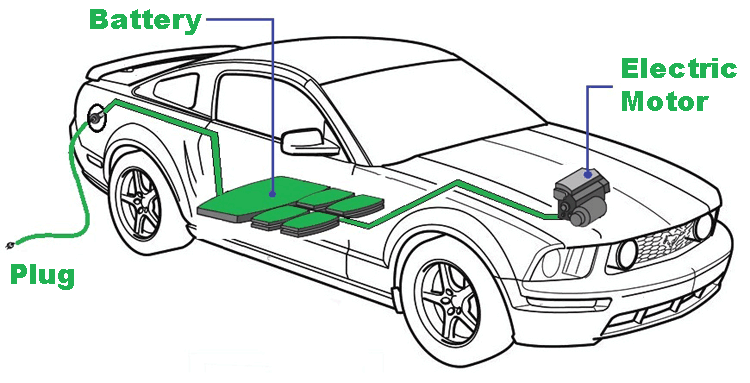
\includegraphics[width=0.7\textwidth]{EV.png}
            \caption{Esquematico de un vehiculo electrico}
            \label{EV}
        \end{center}
    \end{figure}


	\noindent Siendo las baterías eléctricas la única fuente de energía en los 
    VVEE, éstas tienen un gran impacto en la performance de los mismos 
    determinando la autonomía del vehículo. En base a este criterio, las 
    baterías de iones de litio (\emph{Li-Ion}) resultan las más adecuadas para 
    esta aplicación debido a su alta densidad energética, es decir, que éste 
    tipo de baterías tienen una gran capacidad para su reducido volumen a 
    comparación de otras tecnologías. Para poder ser utilizados en VVEE, las 
    baterías de Li-Ion son conectadas en forma de arreglos o packs de baterías 
    en serie que permiten obtener mayores valores de tensión y, otras, en 
    paralelo para aumentar la capacidad del pack. 

    \subsection{Motivacion del proyecto}
	
	\noindent Una de las grandes problematicas de las baterias de Litio-ion 
    reside en que se debe tener en cuenta ciertas precauciones a la hora de
    implementarlas, debido a que las mismas son propensas a fallar al ser 
    sobrecargadas, completamente descargadas u operadas fuera del
    rango seguro de temperatura, tension o corriente, ademas, en un pack de 
    baterias conectadas en serie, se puden manifestar pequeñas diferencias de 
    capacidades a traves de todas las celdas, causado por tolerancias de
    produccion o diferentes condiciones de operacion, que tienden
    a incrementar con cada ciclo de carga. Por ultimo, las baterias
    sufren un proceso de \emph{auto-descarga} (tipicamente entre un
    2-10\% dependiendo de la temperatura y el estado de carga de la misma). 
    Si la distribucion de temperatura a lo largo del pack es
    heterogenea, las celdas con mayor temperatura tienden a una mayor
    perdida de capacidad provocando un desbalanceo de carga.
    Esto trae varias consecuencias, entre ellas, se encuentran:

	\begin{itemize}
		\item \textbf{Seguridad:} Si el voltaje máximo de carga es excedido por 
        unos cientos de milivoltios, puede provocar un embalamiento térmico, 
        derritiendo el pack de baterias y, por lo tanto, el dispositivo que 
        alimenta. En el peor de los casos puede explotar poniendo en riesgo el 
        bienestar del usuario.
		\item \textbf{Salud de la batería:} La degradación de la batería es 
        extremadamente sensible a la operación de la misma fuera de la zona 
        indicada. Si la temperatura de operación o la tensión máxima de carga 
        es excedida esto provoca una aceleración en la degradación de su vida 
        útil.
		\item \textbf{Autonomía:} Consideremos que el circuito de protección 
        detecta que una de las baterías se encuentra descargada a niveles 
        cercanos de operación insegura. En este caso, la protección frena la 
        descarga del pack por una sola celda y el resto se encuentran con 
        voltajes más altos y, por lo tanto, con un remanente de energía para 
        entregar a la carga desaprovechando la capacidad del pack entero.
	\end{itemize}
    
    \noindent Lo que conlleva la implementación de un sistema de administración 
    de baterías. En definitiva, un BMS es un dispositivo encargado de controlar 
    las funciones vitales de las baterías para que operen de forma correcta y 
    segura, con el objetivo de otorgar seguridad al usuario y prolongar la 
    autonomía del vehículo. Las funciones más relevantes que llevan a cabo estos 
    sistemas son:
	
	\begin{itemize}
		\item Protección del pack para su operación en la región segura tanto 
            en tensión, corriente como también en temperatura.
		\item Ecualización de las celdas individuales del pack, es decir,
            controlar que la carga entre celdas sea uniforme
		\item Estimación del estado de carga del pack de batería 
            (\emph{SoC, por sus siglas en inglés State of Charge}).
		\item Estimación del estado de salud del pack de batería 
            (\emph{SoH, por sus siglas en inglés State of Health}).
		\item Informar a la computadora central del vehículo los distintos 
            parámetros del pack de baterías.
	\end{itemize}

    \noindent Ademas de las problematicas mencionadas anteriormente, en el 
    mercado actual se venden una gran variedad de BMS con escaza documentacion  
    sobre el mismo, dificultando su implementacon con otros dispositivos, tales
    como computadoras centrales de vehiculos electricos hasta UPS.

    \noindent Por su contraparte, existen solamente dos proyectos de 
    codigo/hardware abiertos relacionados al desarrollo de BMS, detallados a
    continuacion.

    \subsubsection{foxBMS}

    \emph{foxBMS} es un proyecto desarrollado por el Instituto de Sistemas 
    Integrados y Tecnologias de Dispositivos de la sociedad \emph{Fraunhofer} o 
    tambien llamado Fraunhofer IISB (del ingles \emph{Institute for Integrated 
    Systems and Device Technology IISB}), una organizacion de investigacion 
    alemana que comprende 72 institutos esparcidos por todo el territorio
    aleman.
    
    \noindent El desarrollo de este proyecto es el resultado de 15 años de 
    investigacion en el area de energias renovables y es diseñado para 
    administrar innovadores prototipos de sistemas de bateria basados en la 
    tecnologia iones de litio, desde pocas celdas conectadas en serie hasta 
    centenares de kWh y kW, especialmente para sistemas que requieren niveles 
    de seguridad de alta fiabilidad.
    
    \noindent El proyecto no tiene intenciones de ser usado de forma comercial 
    en productos ya que no cumple con estandards especificos y requieren
    determinados certificados. Solamente cumple con el proposito de ser una
    plataforma de ensayo y desarollo que provee todas las funcionalidades del
    manejo de la complejidad y tamaño de los sistemas de almacenamiento mas
    avanzados al dia de la fecha.
    
    \noindent Si bien el mismo tiene extensa documentacion, originalmente fue
    desarrollado para manejar packs de 12 a 18 celdas en serie, lo cual excede
    el proposito de la aplicacion en cuestion por lo que no resulta viable para
    ser implementado de forma directa. Tambien el hardware del proyecto es
    extensivamente costoso y complejo, ya que implementa varios 
    microcontroladores e integrados dedicados hasta FPGAs 
    (del ingles, \emph{Field Programmable Gate Arrays}).

    \clearpage

    \subsubsection{openBMS}

    A diferencia de \emph{foxBMS}, este proyecto fue desarrollado por 
    ingenieros independientes con el objetivo de diversificar los proyectos 
    abiertos relativos al tema en cuestion.
    
    \noindent Este projecto busca desarrollar un BMS capaz de manejar un pack 
    de baterias de 4 a 96 celdas en serie, realizar el balanceo de las mismas y 
    comunicar las variables del pack a traves del protocolo CAN.
    
    \noindent Si bien, se encuentran todos los archivos del proyecto a 
    disponibilidad del publico, la documentacion es muy escaza 
    para ser implementado facilmente durante el proceso de desarrollo de un
    vehiculo electrico.
    
    \noindent En definitiva, la complejidad en el manejo de grandes packs de 
    baterias basadas en celdas de litio-ion y la falta de proyectos abierto 
    disponibles relacionados al tema, son la fuente de motivacion para 
    llevar a cabo el presente trabajo.
    
    \noindent Finalmente, el informe se encuentra dividido en varias secciones, 
    en la seccion \ref{descripcion} se realiza una descripcion en alto nivel del
    proyecto, detallando los objetivos generales, las especificaciones y
    requerimientos del trabajo, a continuacion de esa seccion, se encuentra el
    fundamento teorico (Seccion \ref{teoria}), donde se detalla el 
    funcionamiento de una celda de litio-ion, desarrollo del modelo de las 
    celdas elegidas, los algoritmos utilizados en el proyecto en conjunto con 
    todo su desarrollo matematico, por ultimo se presentan las secciones 
    \ref{desarrollo} y \ref{ensayos} donde se describe el desarrollo tanto del 
    firmware y hardware del dispositivo en conjunto con los ensayos realizados 
    para validar el dispositivo respectivamente. Finalmente, en la seccion 
    \ref{conclusiones} se desarrollan las conclusiones y futuros proyectos a 
    continuar sobre el eje de estudio.
	
	\clearpage
	
    \section{Descripcion}\label{descripcion}
	
	\subsection{Objetivos Generales}

    Como solucion a los problemas planteados en la seccion anterior, se propone
	desarrollar un BMS que cumpla con los siguientes requisitos:

    \begin{itemize}
        \item Proteger el pack de baterías evitando que el mismo salga de su 
        zona de operación segura, tanto en tensión, corriente como en 
        temperatura evaluando los umbrales correspondientes de operación para 
        las celdas de Litio-Ion.
        \item Estimar el estado de carga en tiempo real utilizando estos datos 
        con el fin de llevar al sistema al punto de operación óptima.
        \item Balancear la carga entre celdas priorizando el menor costo 
        energético posible del sistema y la mayor autonomía final del pack.
        \item Comunicar los parámetros fundamentales del pack a una computadora 
        central a través de algún protocolo estandarizado.
    \end{itemize}

	\noindent Para lograr estos objetivos, se plantea un estudio pormenorizado 
    del estado del arte de la temática en cuestión procurando seleccionar las 
    prácticas y metodologías más adecuadas para la solución del problema 
    planteado, a partir de un estudio teórico. Finalmente se validará la 
    solución elegida a partir de la implementación y ensayo de la solución 
    desarrollada.
	
	\subsection{Especificaciones}

    \noindent El sistema a implementar debe ser capaz de poder administrar un 
    pack de baterias de 6 modulos conectados en serie, donde cada modulo esta 
    compuesto por 3 celdas en paralelo encargado de: 
	
	\begin{itemize}
		\item Sensar la tensión de las celdas individuales del pack y de la 
        corriente que circula desde y hacia el pack asi, como tambien 
        la temperatura media.
		\item Realizar el balanceo de los modulos que componen la bateria.
		\item Proteger el mismo, desconectando el pack de baterias de la carga
            frente a operaciones fuera de la zona segura.
		\item Estimar el estado de carga y detectar las celda que se encuentran
            en desbalance utilizando una unidad de computo como por ejemplo, un
            microcontrolador o MCU (del ingles \emph{Microcontroller Unit}).
        \item Controlar el proceso de carga del pack de bateria
        \item Comunicar las variables del sistema a una computadora central a
        traves de un protocolo especificado
	\end{itemize}
	
	\noindent La descripción anterior se puede visualizar en el Diagrama de 
    Bloques (DB) de la Figura \ref{bms}. Como puede observarse, 
    el microcontrolador es el encargador de comunicarse y comandar los modulos 
    de proteccion, ecualizacion y carga de la bateria, como tambien obtener 
    variables de los mismos para poder estimar el SoC, determinar el 
    desbalanceo de una o mas celdas y tomar accion al respecto, y por ultimo, 
    pero mas relevante, comandar las protecciones en caso de una falla y/o 
    alerta de la bateria. De forma simultanea, el mismo debe estar a cargo de 
    comunicar las distintas variables del sistema a una computadora central.

    \clearpage

	\begin{figure}[h!]
		\begin{center}
			\begin{circuitikz}[european]
				\draw (-4, -1) rectangle (-2, 1)[fill=blue!10!white];
				\node at (-3, 0.2) {CPU};
				\node at (-3, -0.2) {Central};
				\draw [vecArrow] (-1.8, 0) to (-1, 0);
				\draw [vecArrow] (-1.2, 0) to (-2, 0);
				
				\draw (-1, -1) rectangle (1, 1)[fill=blue!10!white];
				\node at (0, 0) {MCU};
				
				\draw [blue,thin,dashed] (2.1, 2.5) rectangle (5.1, -2.5)[fill=blue!10!white];
				
				\draw (2.2, 2.4) rectangle (5.0, 0.92)[fill=yellow!15!white];
				\draw (2.2, 0.82) rectangle (5.0, -0.71)[fill=yellow!15!white];
				\draw (2.2, -0.81) rectangle (5.0, -2.4)[fill=yellow!15!white];
				
				
				
				\node at (3.6, 1.6) {Protección};			
				\node at (3.6, -1.6) {Cargador};
				\node at (3.6, 0) {Equalizacion};
				\draw [vecArrow] (1.2, 0) to (2.1, 0);
				\draw [vecArrow] (1.5, 0) to (1, 0);
				
				\draw (7, 2) -- (7, 2.2);
				\draw (7, 2) to[battery1] (7, 1.6);
				\draw (7, 1.4) -- (7, 1.6);
				\draw (7, 1.4) to[battery1] (7, .9);			
				\draw (7, .7) -- (7, .9);			
				\draw (7, 0.7) to[battery1] (7, 0.2);			
				\draw (7, 0.2) -- (7, -0.2);
				\draw (7, -0.2) to[battery1] (7, -0.7);
				\draw (7, -.7) -- (7, -.9);
				\draw (7, -.9) to[battery1] (7, -1.4);
				\draw (7, -1.4) -- (7, -1.6);
				\draw (7, -1.6) to[battery1] (7, -2);
				\draw (7, -2) -- (7, -2.2);
				
				\draw (9, 2) -- (9, 2.2);
				\draw (9, 2) to[battery1] (9, 1.6);
				\draw (9, 1.4) -- (9, 1.6);
				\draw (9, 1.4) to[battery1] (9, .9);			
				\draw (9, .7) -- (9, .9);			
				\draw (9, 0.7) to[battery1] (9, 0.2);			
				\draw (9, 0.2) -- (9, -0.2);
				\draw (9, -0.2) to[battery1] (9, -0.7);
				\draw (9, -.7) -- (9, -.9);
				\draw (9, -.9) to[battery1] (9, -1.4);
				\draw (9, -1.4) -- (9, -1.6);
				\draw (9, -1.6) to[battery1] (9, -2);
				\draw (9, -2) -- (9, -2.2);
				
				\draw (11, 2) -- (11, 2.2);
				\draw (11, 2) to[battery1] (11, 1.6);
				\draw (11, 1.4) -- (11, 1.6);
				\draw (11, 1.4) to[battery1] (11, .9);			
				\draw (11, .7) -- (11, .9);			
				\draw (11, 0.7) to[battery1] (11, 0.2);		
				\draw (11, 0.2) -- (11, -0.2);
				\draw (11, -0.2) to[battery1] (11, -0.7);
				\draw (11, -.7) -- (11, -.9);
				\draw (11, -.9) to[battery1] (11, -1.4);
				\draw (11, -1.4) -- (11, -1.6);
				\draw (11, -1.6) to[battery1] (11, -2);
				\draw (11, -2) -- (11, -2.2);
				
				
				\draw (5.1, 0) to[short, -*] (7, 0);
				\draw (7, 0) to[short, -*] (9, 0);
				\draw (9, 0) to[short, -*] (11, 0);
				
				\draw (7, 0.8) to[short, -*] (9, 0.8);
				\draw (9, 0.8) to[short, -*] (11, 0.8);
				
				\draw (7, 1.5) to[short, -*] (9, 1.5);
				\draw (9, 1.5) to[short, -*] (11, 1.5);
				
				\draw (7, 2.2) to[short, -*] (9, 2.2);
				\draw (9, 2.2) to[short, -*] (11, 2.2);			
				
				\draw (7, -0.8) to[short, -*] (9, -0.8);
				\draw (9, -0.8) to[short, -*] (11, -0.8);
				
				\draw (7, -1.5) to[short, -*] (9, -1.5);
				\draw (9, -1.5) to[short, -*] (11, -1.5);
				
				\draw (7, -2.2) to[short, -*] (9, -2.2);
				\draw (9, -2.2) to[short, -*] (11, -2.2);			
				
				\draw (5.1, 0.2) -- (6.2, 0.2) |- (7, 0.8) node at (7, .8){$\bullet$};
				\draw (5.1, 0.4) -- (6, 0.4) |- (7, 1.5) node at (7, 1.5){$\bullet$};
				\draw (5.1, 0.6) -- (5.8, 0.6) |- (7, 2.2) node at (7, 2.2){$\bullet$};
				
				\draw (5.1, -0.2) -- (6.2, -0.2) |- (7, -0.8) node at (7, -.8){$\bullet$};
				\draw (5.1, -0.4) -- (6, -0.4) |- (7, -1.5) node at (7, -1.5){$\bullet$};
				\draw (5.1, -0.6) -- (5.8, -0.6) |- (7, -2.2) node at (7, -2.2){$\bullet$};
				
				\draw [dashed] (-1.2, 2.6) rectangle (5.2, -2.6);
				\draw node at (-.8, 2.8){BMS};
				
				\draw [dashed] (6.5, 2.4) rectangle (11.5, -2.4);
				
				\draw node at (8.2, 2.6) {Pack de Baterías 6s3p};
				
				
				
				\draw (13, 1) to[R=$Z$] (13, -1);
				
				\draw (11, 2.2) -- (12, 2.2)
				|- (12, 1.5) -- (13, 1.5) |- (13,1) node at (12, 1.5){$\bullet$};
				
				\draw (11, -2.2) -- (12, -2.2)
				|- (12, -1.5) -- (13,-1.5) |- (13,-1) node at (12, -1.5){$\bullet$};
				
				
				
				\draw node at (12.8, 1){+};
				\draw node at (12.8, -1){-};
				
				
			\end{circuitikz}
		\end{center}
		\caption{Diagrama en Bloques del BMS y el pack de baterías}
		\label{bms}
	\end{figure}

	\clearpage
	
    \section{Aspectos Teoricos}\label{teoria}
	
	\subsection{Batería de Litio-Ion}
    
    La energia electrica ha empoderado a la sociedad desde su 
    descubrimiento y, gracias a sus avances tecnologicos, el acceso a la misma 
    se ha convertido mas facil y mas eficiente, aun asi con la
    ausencia de conexiones electricas en la cercania. Sumado a eso, tambien
    nos dirigimos a una sociedad que aprovecha de la movilidad a medida que los
    dispositivos dependen menos de una conexion electrica local.\\
    \\
    \noindent En gran parte, estos desarrollos son posibles gracias al
    descubrimiento del litio-ion y su aplicacion en baterias. Este tipo de
    bateria ha revolucionado la tecnologia en almacenamiento de energia y ha
    logrado impulsar la revolucion digital empoderando los dispositivos moviles,
    a traves de su gran capacidad y densidad energetica.

    \subsubsection{Principios basicos}

    El principio basico de funcionamiento de una bateria, en su configuracion
    basica, consiste en \emph{(fig. \ref{batt_wk_ppl})} una celda 
    compuesta por dos electrodos, cada una conectada a un circuito 
    electrico, separado por un electrolito que es capaz de acomodar cargas
    dentro de si. Frecuentemente, los electrodos son fisicamente separados por
    una barrera que previene que esten en contacto fisico entre si, evitando asi
    un corto circuito en la bateria. En descarga, cuando la bateria
    entrega corriente al circuito, toma lugar un proceso de oxidacion en el
    electrodo negativo (anodo), resultando en un movimiento de electrones a
    traves del circuito. Por el otro lado, en el electrodo positivo (catodo),
    ocurre un proceso de reduccion, reabastecido por los electrones del
    circuito. El voltage de la celda depende fuertemente de la diferencia de
    potencial entre los electrodos, y del proceso espontaneo en su totalidad.
    Para baterias recargables el proceso puede ser reversible aplicando
    electricidad externa produciendo un proceso complementario de \emph{redox}
    (reduccion-oxidacion) en los electrodos. Este proceso es dependiente de la
    energia y es no espontaneo, es decir, que sucedera si y solo si un agente
    externo participa en el proceso.

    \begin{figure}[h!]
        \begin{center}
            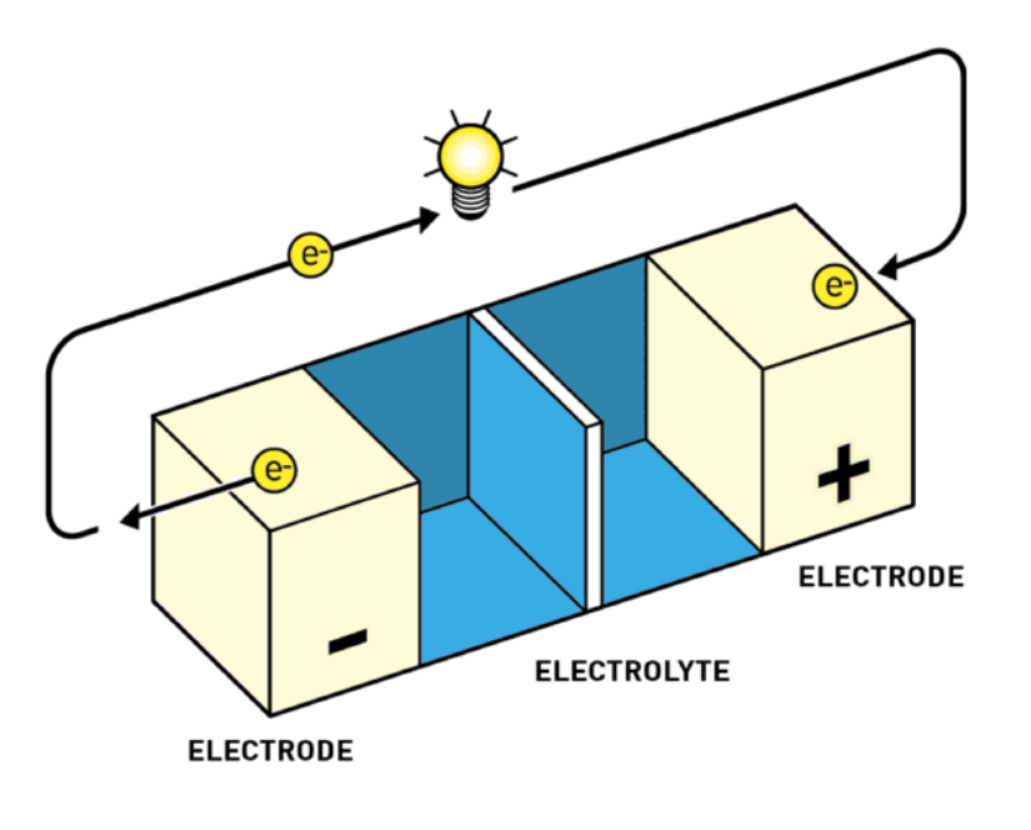
\includegraphics[width=0.4\textwidth]{batt_func_ppr.png}
        \end{center}
        \caption{Principio basico de funcionamiento de una bateria en el
        proceso de descarga. Procesos de \emph{redox} resultan en corriente
        electrica ciruclando a traves del circuito. Durante el proceso de
        carga, se da un proceso de \emph{redux} dado por un agente externo 
        que entrega electricidad en los electrodos resultadno en un proceso
        espontaneo reversible.}
        \label{batt_wk_ppl}
    \end{figure}

    \clearpage

    \noindent En base a este principio de funcionamiento, surgen una gran 
    variedad de tecnologias, partiendo de la pila voltaica, hecha de dos discos
    de metales distintos, uno de zinc y otro de cobre o plata, separados por un
    dielectrico (como carton o cuero) sumergido en una solucion electrolitica.
    Durante la operacion, el disco de zinc actua como anodo, liberando
    electrones al circuito y produciendo iones de metal (proceso de oxidacion),
    mientras que la reaccion en el electrodo opuesto depende de las condiciones
    de trabajo. En la presencia del aire, el metal de cobre es parcialmente
    oxidado a CuO, y la reduccion de CuO a Cu se da en el electrodo. En la
    ausencia de aire, los protones en el electrolito son reducidos a hidrogeno
    en la superficie del cobre. El voltage de la celda es de aproximadamente
    0.8-1.1V, dependiendo de la exposicion al aire. Esencialmente, la pila
    voltaica fue una bateria no recargable. 
    
    \noindent Despues surgieron las baterias de plomo-acido, que tiene un 
    principio de funcionamiento similar a las baterias voltaicas expuestas al 
    aire, pero con la posibilidad de ser recargadas. Esta tecnologia se basa en 
    dos electrodos de plomo, donde uno se encuentra parcialmente oxidado a 
    oxido de plomo ($\mathrm{PbO_2}$), separado por acido sulfurico que contiene un 
    electrolito. Durante el proceso de descarga, ocurre un proceso de oxidacion 
    en el electrodo de plomo (anodo), produciendo electrones, protones y 
    sulfato de plomo ($\mathrm{PbSO_4}$), mientras que el oxido de plomo es 
    reducido a $\mathrm{PbSO_4}$ en el catodo. En este caso, el potencial de 
    una celda es de alrededor 2V.
    
    \noindent Otro logro en el desarrollo de baterias, ocurrio en el 1899 cuando 
    se desarrollo la primer bateria de niquel-hierro (Ni-Fe) y niquel-cadmio
    (Ni-Cd) o tambien conocidas como baterias alcalinas, que fueron
    predecedoras del hibrido niquel-metal (Ni-MH) que fue comercializada en
    1898.
    
    \noindent Las baterias anteriores son basadas en soluciones acuosas, y la
    densidad energetica de las mismas no es alta, especificamente son menores a
    los 100Wh/kg. Para incrementar la densidad energetica de estas baterias, es necesario
    encontrar una estabilidad electroquimica del agua ya que juega un rol muy
    importante en ello. Ademas, cuando ambos electrodos utilizando el alto 
    potencial del plomo, el voltage de salida solo puede alcanzar un voltage 
    maximo de 2.2V. Como resultado, con la necesidad de incrementar la densidad
    energetica de una celda, se descubrio el metal de litio y su aplicacicacion
    en las celdas de litio.


    \subsubsection{Litio}

    El litio es un metal descubierto en 1818 que tiene excelentes 
    propiedades para servir como material para el desarrollo de baterias. 
    Es el metal mas liviano con una densidad de 0.53$\mathrm{g/cm^3}$. 
    Tambien tiene un potencial de reduccion muy bajo, que lo hace ideal para 
    celdas de alta densidad y alto voltage. Sin embargo, es un metal 
    reactivo que debe ser protegido, por ejemplo, del agua y del aire, 
    ya que el contacto con estos provoca que el mismo sea muy complicado de 
    dominar, imposibilitando su uso para la aplicacion deseada. 
    Esta proteccion al medio no es trivial, y factores, tales como 
    su caracter inerte, punto de fusion, la estabilidad del \emph{redox}, 
    solubilidad de iones de litios y sales, velocidades de transferencia 
    ion/electron, viscosidad, entre otros deben ser considerados.
    
    \noindent Las primeras baterias de litio alcanzaron el mercado en 1970 y la 
    comercialización de las mismas comenzó en Japón en el año
    1991, cuando \emph{Sony Corporation} presento el primer modelo.
    
	\noindent Las baterías de litio-ion son definidas en \cite{def_liion} como 
    almacenadores de energía que utilizan iones de Litio como portadores de 
    carga. En base a esta definición, el término \emph{batería de Litio-Ion} no 
    se corresponde con una sola composición química, como lo son las baterías 
    de ácido o niquel-cadmio, si no que expresa una familia de baterías que 
    dependen de los iones de Litio pero que pueden ser conformadas por 
    distintos materiales.
    
    \noindent A diferencia de las baterías de ácido, hay dos razones principales por las 
    cuales las baterías de Litio-ion han crecido en popularidad en tan poco 
    tiempo: su excelente rendimiento y la capacidad de adaptarse al creciente 
    mercado de la electrónica de consumo, como por ejemplo, videograbadoras, 
    celulares y computadoras. A partir de la primer década del siglo XXI, se 
    comenzaron a utilizar en vehículos eléctricos, como también en grandes 
    sistemas de almacenamiento de energía, capaces de alimentar barrios 
    residenciales enteros.
    
    \noindent Desde Desde el 2000 al presente, se desarrollaron varios
    tipos de baterias basadas en el litio. Entre ellas se encuentran las
    baterias de litio-sulfuro (Li-S) y litio-aire (Li-air), cuya densidad
    energetica teorica ronda los 2600 Wh/kg y 11400 Wh/kg, repectivamente. En
    2012, se desarrollo una bateria de litio-ion recargable acuosa o ARLB (del
    ingles \emph{Aqueous rechargeable lithium batteries}), 
    que utiliza metal de litio recubierto como anodo en una solucion de 
    electrolitos mejorando ampliamente la densidad energetica.

    \subsubsection{Principio de funcionamiento}

    El principio de los procesos de carga y descarga en las baterias de
    litio-ion se basan en utilizar oxido de litio-cobalto ($\mathrm{LiCoO_2}$)
    y grafito como tipicos materiales de electrodo. La Figura
    \ref{op_lithium-ion} ilustra el princio de operacion, y las reacciones de
    los electrodos se expresan en  las Ecuaciones \ref{li_anode}, 
    \ref{li_catode} y \ref{li_total}

    \reaction{\text{Electrodo positivo: } LiCoO2 <=>[Carga][Descarga] Li_{1-x}CoO2 + xLi + xe^- \label{li_anode}}
    \reaction{\text{Electrodo negativo: }6C + xLi^+ + xe^- <=>[Carga][Descarga] Li_{x}C6 \label{li_catode}}
    \reaction{\text{Reaccion total: }6C + LiCoO2 <=>[Carga][Descarga] Li_{x}C6 + Li_{1-x}CoO2 \label{li_total}}

    \noindent El \ce{LiCoO2} tiene una estructura reticular octaedrica con un arreglo
    alternativo de capas de \ce{Li+} y \ce{Co^{3+}}. Durante el proceso de
    carga, los iones de litio (en estado ionico) se desintercalan de la
    estructura de capas del material del electrodo positivo, liberando electrones, 
    al mismo tiempo, el \ce{Co^{3+}} se oxida convirtiendose en \ce{Co^{4+}}.
    Por el otro lado, durante el proceso de descarga, con la intercalacion de \ce{Li+} dentro de 
    la reticula, el \ce{Co^{4+}} es reducido a \ce{Co^{3+}}, ganando 
    electrones, ademas se obtienen electrones de la reticula para 
    convertirse en litio en estado atomico. Durante este proceso, el estado 
    atomico del litio pierde electrones convirtiendose en iones de litio 
    , este proceso se puede resumir en que el anodo provee al electrodo positivo 
    iones de litio. Dado que el litio se mueve entre el electrodo positivo y 
    negativo hacia ambos lados a este tipo de baterias se las denomina, como 
    una bateria mecedora (del ingles, \emph{rocking chair}).


    \begin{figure}[h!]
        \begin{center}
            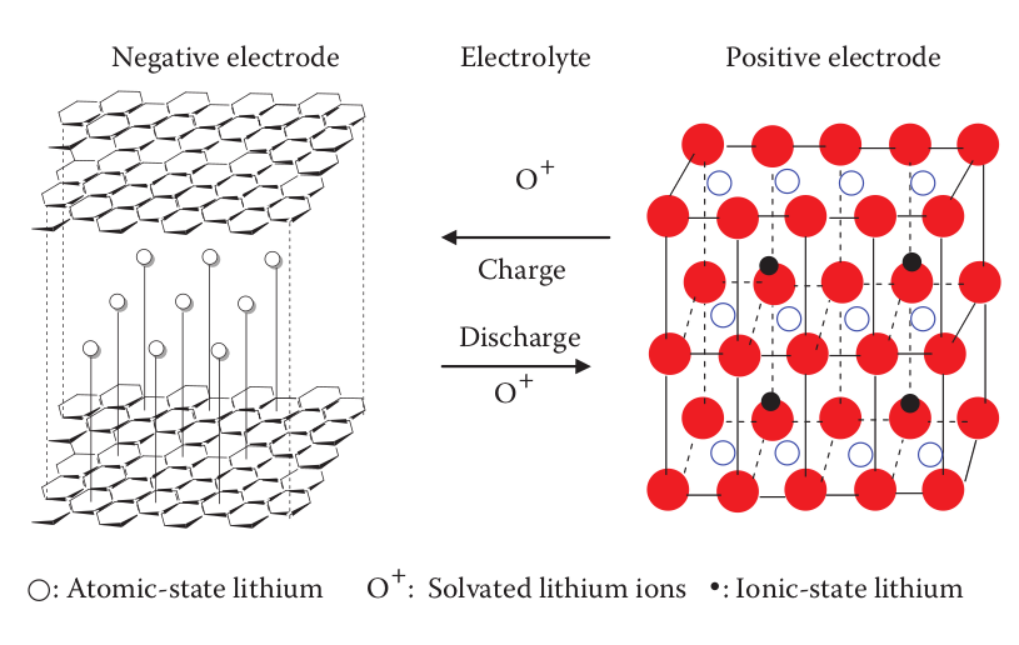
\includegraphics[width=0.7\textwidth]{prin_litio}
            \caption{Esquematico del prinicipio de operacion de una bateria de
            litio-ion.}
            \label{op_lithium-ion}
        \end{center}
    \end{figure}

    \noindent La mayoría de estas baterias usan materiales de carbón, 
    tales como el grafito y el carbón duro como ánodo, otros utilizan óxidos de 
    metales, como por ejemplo, el Titanato de Litio ($\mathrm{Li_4Ti_5O_{12}}$) 
    y el Pentóxido de Niobio ($\mathrm{Nb_2O_5}$), debido a que pueden aceptar 
    iones de Litio cuando son cargados, y liberarlos en el proceso de descarga, 
    estas reacciones se denominan como inserción y extracción respectivamente. 
    Los potenciales de reacción de estos materiales son mucho más bajos que los 
    electrodos de hidrógeno estándares, por lo tanto, el electrolito debería ser 
    estable inclusive para niveles de potencial tan bajos. Ésta es la razón por la 
    cual, los electrolitos orgánicos, que consisten de solventes orgánicos y 
    sales de litio, son utilizados en las baterías de Litio-ion en vez de 
    electrolitos acuosos.
	\clearpage
	\noindent El material activo del cátodo debe contener Litio en su composición química 
    para proveer una fuente de iones de Litio. Durante la primer etapa de 
    desarrollo de las celdas de litio, se utilizaba Óxido de Litio-Cobalto.
    También se estudió el uso de $\mathrm{LiNiO_2}$ como 
    material activo para el cátodo pero fue inmediatamente descartado debido a 
    su inestabilidad térmica. Sin embargo, se desarrollaron y utilizaron 
    derivativos de esta composición, formulados como 
    $\mathrm{LiM_xNi_{1-x}O_2}$ (M: elemento metálico tales como, el Co, Mn, 
    Al, Mg).
	
    Comparada con las baterias de litio-ion originales en los principios de
    1990, el rendimiento de las mismas ha sido mejorado de forma significativa
    con el paso del tiempo. Los ultimos desarrollo tienen ventajas dominantes
    sobre las baterias recargables tradicionales:
	\begin{itemize}
        \item \textbf{Alta densidad energetica:} La densidad energetica por
            volumen y masa para una bateria de litio modelo 18650 puede alcanzar
            los 500 Wh/$\mathrm{dm^3}$ y 230 Wh/kg, respectivamente, que ademas
            se encuentra en continuo aumento a medida que se investigan y
            desarrollan nuevas tecnologias.
        \item \textbf{Alto voltaje de salida (~3.6V):} Esto es 3 veces mayor a
            las baterias recargables de Ni-Cd o Ni-MH.
        \item \textbf{Alta potencia de salida:} Pueden alcanzar hasta 2kW/kg for
            un corto periodo de tiempo.
        \item \textbf{Baja auto-descarga:} La descarga media de las celdas de
            litio son menores a un 3\% mensuales, que es la mitad que las celdas
            basadas en Ni-Cd y Ni-MH.
        \item \textbf{bajo efecto de histeress} A diferencia de las celdas de
            Ni-Cd y Ni-MH las celdas de litio tienen un efecto de histeresis
            despreciable con el paso de los ciclos de carga-descarga de la
            misma, resultando en un mejor ciclo de vida con respecto a los otros
            tipos de celdas.
        \item \textbf{Ciclos de carga-descarga rapidos:} Las baterias de
            litio-ion pueden ser cargadas con corrientes de hasta un 80\% de su
            capacidad. Es decir, si la bateria tiene una capacidad de 3Ah, la
            misma se puede cargar a una corriente de 3A.
        \item \textbf{Alta eficiencia culombica:} La eficiencia culombica o EC,
            es un parametro que permite obtener que porcentaje del material
            activo se convierte en energia. Su medicion es importante porque 
            permite medir el desempeño de la bateria con respecto a otras 
            tecnologias. En el caso de las celdas de Litio-ion, la eficiencia 
            culombica se mantiene casi en un 100\% inclusive despues del primer
            ciclo.
        \item \textbf{Gran rango de temperaturas}: Las baterias de litio-ion
            pueden operar entre -25\degree C a +45\degree C. Las
            investigaciones actuales quieren extender ese rango desde
            -40\degree C a +70\degree C con mejoras en el
            electrolito y los materiales de los electrodos.
		\item \textbf{} Esto depende fuertemente del 
        alto voltaje, porque la energía específica es el producto del voltaje 
        de la celda y su capacidad específica, lo que hace que las celdas de 
        Litio-Ion se destaquen a comparación de otras tecnologías, 
        como por ejemplo, las celdas de Niquel-metal con un voltaje de 1.2V 
        pero con mayor capacidad tienen menor energía específica. 
		\item \textbf{Alta eficiencia energética:} Esto se debe a dos 
        factores principales, por un lado se debe a la alta eficiencia de 
        carga y descarga debido a que no hay pérdidas durante las reacciones 
        químicas de la celda en ambos procesos y, nuevamente, esto se atribuye 
        también a su alto voltaje. Éste último, se debe a que la eficiencia 
        energética, es el restante de la tensión operativa en relación a la 
        tensión en circuito abierto. Suponiendo que tenemos una celda A con una 
        tensión de circuito abierto ($\mathrm{V_A}$) mayor que otra celda B con 
        una tensión $\mathrm{V_B}$, que tiene la misma pérdida de voltaje X, 
        la eficiencia de A va a ser mayor que la de B, dado por:
		
		\clearpage
		\begin{equation}
			\frac{V_A - X}{V_A} > \frac{V_B - X}{V_B} \nonumber
		\end{equation}
		\item \textbf{Larga duración:} Esto se atribuye a que las reacciones 
        dentro de la celda, durante los ciclos de carga y descarga, no realizan 
        cambios morfológicos significativos. Esto es bastante distinto con las 
        baterías de ácido, donde la reacción que se lleva a cabo involucra la 
        disolución y deposición de materiales, lo que representa grandes 
        cambios morfológicos durante los ciclos de carga y descarga.
		
	\end{itemize}
	
	\noindent Por último, las baterías de Litio-ion utilizan electrolitos 
    orgánicos. El electrolito permite que la celda tenga alto niveles de 
    tensión, sin embargo la combustibilidad del mismo genera problemas de 
    seguridad. Por lo tanto, es clave para el desarrollo de estas baterías 
    minimizar la causa y efecto de la combustión de la misma sin sacrificar 
    rendimiento.
	
	\noindent El estado de las baterías de Litio-ion con respecto a las otras 
    tecnologías se puede observar en la Figura \ref{comparisson_batt}, donde se 
    puede observar la dominancia de las mismas sobre el resto de las 
    tecnologías, en términos de densidad energética (Wh/L) y energía específica 
    (Wh/kg). La flecha de la esquina derecha indica que ésta tecnología se 
    encuentra en constante desarrollo y puede mejorar con el paso del tiempo.

    \begin{figure}[h!]
        \begin{center}
            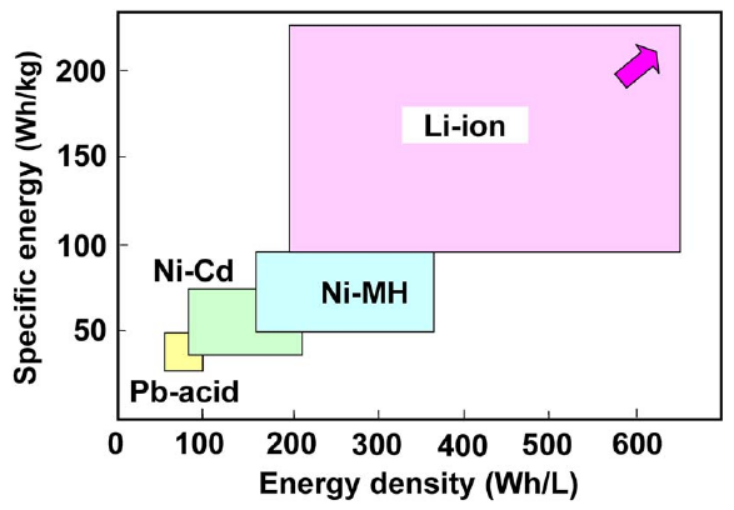
\includegraphics[width=0.7\textwidth]{comparisson-liion.png}
            \caption{Grafica comparativa entre distintas
            tecnologias de baterias.}
            \label{comparisson_batt}
        \end{center}
    \end{figure}

	\noindent La aplicación práctica de las baterías de Litio-ion involucra la 
    integración de las mismas dentro de un sistema, involucrando un controlador 
    central (BMS), sistemas de refrigeración, sensores y conectores entre las 
    celdas. En este sistemas las celdas pueden conectarse de distintas 
    formas, por ejemplo, pueden conectarse en paralelo, para incrementar la 
    capacidad del pack, en serie, para incrementar el voltaje, o combinadas 
    para lograr ambos cometidos al mismo tiempo. Por ejemplo, un auto eléctrico 
    de la marca \emph{Tesla}, posee un pack de baterías de 85KWh compuesto por 
    7104 celdas, con una arquitectura de 16 modulos conectados en serie, 
    donde cada uno posee 444 celdas conectadas en paralelo.

    \clearpage

	\noindent En este caso utilizaremos celdas de Litio-ion modelo NCR18650PF, 
    integrando una arquitectura \emph{6S3P}, es decir, 6 modulos conectados en 
    serie donde cada uno esta compuesto por 3 celdas conectadas en paralelo. 
    En la Figura \ref{pack} se muestra el esquemático de la arquitectura del 
    pack como también una foto de la celda que se utilizará para conformar el 
    pack. 
	
	\begin{figure}[h!]
		\begin{minipage}[c]{0.45\textwidth}
			\centering
			\begin{circuitikz}[european]
				
				\draw (7, 2) -- (7, 2.2);
				\draw (7, 2) to[battery1] (7, 1.6);
				\draw (7, 1.4) -- (7, 1.6);
				\draw (7, 1.4) to[battery1] (7, .9);			
				\draw (7, .7) -- (7, .9);			
				\draw (7, 0.7) to[battery1] (7, 0.2);			
				\draw (7, 0.2) -- (7, -0.2);
				\draw (7, -0.2) to[battery1] (7, -0.7);
				\draw (7, -.7) -- (7, -.9);
				\draw (7, -.9) to[battery1] (7, -1.4);
				\draw (7, -1.4) -- (7, -1.6);
				\draw (7, -1.6) to[battery1] (7, -2);
				\draw (7, -2) -- (7, -2.2);
				
				\draw (9, 2) -- (9, 2.2);
				\draw (9, 2) to[battery1] (9, 1.6);
				\draw (9, 1.4) -- (9, 1.6);
				\draw (9, 1.4) to[battery1] (9, .9);			
				\draw (9, .7) -- (9, .9);			
				\draw (9, 0.7) to[battery1] (9, 0.2);			
				\draw (9, 0.2) -- (9, -0.2);
				\draw (9, -0.2) to[battery1] (9, -0.7);
				\draw (9, -.7) -- (9, -.9);
				\draw (9, -.9) to[battery1] (9, -1.4);
				\draw (9, -1.4) -- (9, -1.6);
				\draw (9, -1.6) to[battery1] (9, -2);
				\draw (9, -2) -- (9, -2.2);
				
				\draw (11, 2) to[battery1] (11, 1.6);
				\draw (11, 1.4) -- (11, 1.6);
				\draw (11, 1.4) to[battery1] (11, .9);			
				\draw (11, .7) -- (11, .9);			
				\draw (11, 0.7) to[battery1] (11, 0.2);		
				\draw (11, 0.2) -- (11, -0.2);
				\draw (11, -0.2) to[battery1] (11, -0.7);
				\draw (11, -.7) -- (11, -.9);
				\draw (11, -.9) to[battery1] (11, -1.4);
				\draw (11, -1.4) -- (11, -1.6);
				\draw (11, -1.6) to[battery1] (11, -2);
				\draw (11, -2) -- (11, -2.2);
				
				\draw (7, 0) -- (9, 0);
				\draw (9, 0) -- (11, 0);
				
				\draw (7, 0.8) -- (9, 0.8);
				\draw (9, 0.8) -- (11, 0.8);
				
				\draw (7, 1.5) -- (9, 1.5);
				\draw (9, 1.5) -- (11, 1.5);
				
				\draw (7, 2.2) -- (9, 2.2);
				\draw (9, 2.2) -- (11, 2.2);			
				
				\draw (7, -0.8) -- (9, -0.8);
				\draw (9, -0.8) -- (11, -0.8);
				
				\draw (7, -1.5) -- (9, -1.5);
				\draw (9, -1.5) -- (11, -1.5);
				
				\draw (7, -2.2) -- (9, -2.2);
				\draw (9, -2.2) -- (11, -2.2);			
				
				\draw [dashed] (6.5, 2.4) rectangle (11.5, -2.4);
				
				\draw node at (8.2, 2.6) {Pack de Baterías 6s3p};
			\end{circuitikz}
		\end{minipage}
		\begin{minipage}[c]{0.45\textwidth}
			\centering
			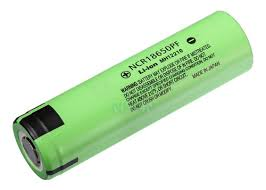
\includegraphics[width=0.75\textwidth]{18650.jpg}
		\end{minipage}
		\caption{A la izquierda se visualiza el esquemático de la arquitectura 
        del pack de baterías. A la derecha se muestra una foto de una celda 
        NCR18650PF.}
		\label{pack}
	\end{figure}
	
    \noindent Estas celdas se caracterizan por su cátodo, cuya composición 
    química se basa en el óxido de Litio Niquel Cobalto Aluminio 
    ($\mathrm{LiNiCoAlO_2}$) y, según sus hojas de datos 
    \cite{18650_datasheet}, sus carateristicas electricas se 
    pueden observar en la Tabla \ref{ncr_table}.
	
	\begin{table}[h!]
		\begin{center}
			\begin{tabular}{|c|l|}
				\hline
                \multicolumn{2}{|c|}{Especificaciones elecctricas}                          \\ \hline
				\textbf{Capacidad Específica}                 & 2700mAh                            \\ \hline
				\multirow{2}{*}{\textbf{Capacidad}}           & Mínimo: 2750mAh                    \\ \cline{2-2} 
				& Tipico: 2900mAh                    \\ \hline
				\textbf{Corriente de Descarga Máxima}         & 10000mAh($\sim$3.5C)               \\ \hline
				\textbf{Rango operativo de tensión}           & 2.5V - 4.2V                        \\ \hline
				\textbf{Voltaje Nominal}                      & 3.6V                               \\ \hline
				\textbf{Charga}                               & CC-CV, Std. 1375mA, 4.20V, 4.0 hrs \\ \hline
				\textbf{Peso}                                 & 48g                              \\ \hline
				\multirow{3}{*}{\textbf{Temperatura}}         & Carga: 0 a 45C                     \\ \cline{2-2} 
				& Descarga: -20 a 60C                \\ \cline{2-2} 
				& Almacenaje: -20 a 50C              \\ \hline
				\multirow{2}{*}{\textbf{Densidad Energética}} & Volumetrica: 577Wh/l               \\ \cline{2-2} 
				& Gravimetrica: 207wh/kg             \\ \hline
			\end{tabular}%
            \caption{Especificaciones electricas de una celda de litio NCR18650PF}
            \label{ncr_table}
		\end{center}
	\end{table}
	
	\noindent Por el otro lado, la hoja de datos también nos provee curvas 
    significativas, como por ejemplo, la curva de carga 
    \emph{(Fig. \ref{cc_cv})}, la curva de descarga para distintas corrientes 
    \emph{(Fig. \ref{descarga_18650})} y la curva del ciclo de vida típico de 
    la batería \emph{(Fig. \ref{life_cycle_18650})}.

    \clearpage
	
	\begin{figure}[h!]
		\begin{center}
			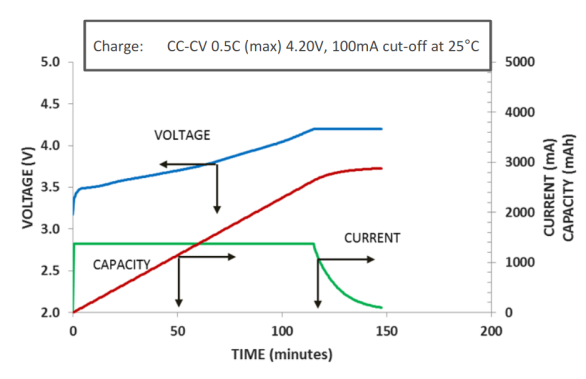
\includegraphics[width=0.8\textwidth]{cc_cv_18650.png}
			\caption{Curva de carga.}
			\label{cc_cv}
		\end{center}
	\end{figure}
	
	\begin{figure}[h!]
		\begin{center}
			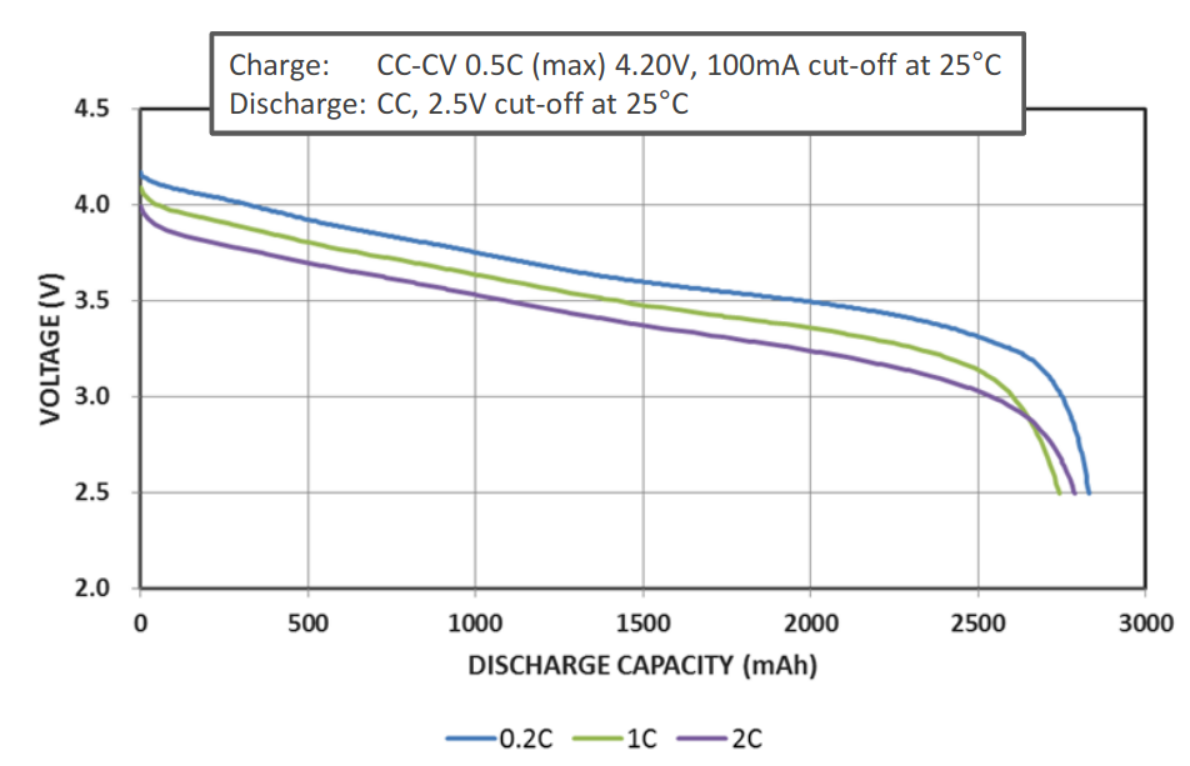
\includegraphics[width=0.8\textwidth]{discharge_18650.png}
			\caption{Curva de descarga en base a distintas corrientes de descarga (0.5C, 1C, 1.5C y 2C)}
			\label{descarga_18650}
		\end{center}
	\end{figure}

    \clearpage
	
	\begin{figure}[h!]
		\begin{center}
			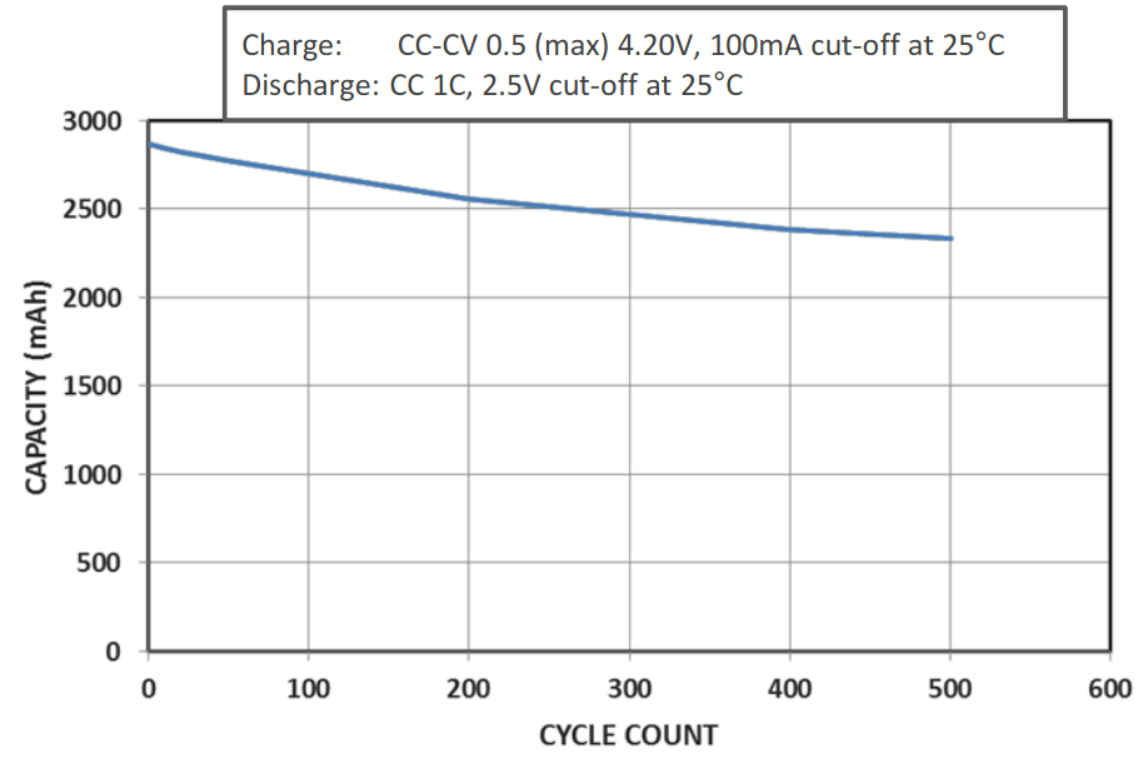
\includegraphics[width=0.7\textwidth]{life_cycle_18650.png}
			\caption{Curva del ciclo de vida de una celda 18650}
			\label{life_cycle_18650}
		\end{center}
	\end{figure}
	
	%TODO La sección debería ser incluida en la descripción del hardware o PCB del BMS
	
	\subsection{Sensado de Corriente}
	
	El sensado de la corriente de carga como de descarga del 
    pack de batería juega un rol muy importante en el desarrollo exitoso de un 
    BMS. Es a partir de conocer con precisión la magnitud de corriente que el 
    sistema podrá mantener el pack de baterías operando dentro de la zona 
    segura (SOA por sus siglas en ingles), monitorear la distribución de carga 
    entre las celdas, implementar correctamente los algoritmos de ecualización 
    de carga y mantener un seguimiento preciso del estado de carga.
	
	\noindent Existen en el mercado una gran variedad de tecnologías y 
    soluciones para la medición de corriente en las diferentes aplicaciones. 
    Algunas de las tecnologías mas relevantes, disponibles en el mercado son:
	\begin{itemize}
		\item [] Resistencia Shunt
		\item [] Transformadores de intensidad (TI)
		\item [] Bobina de Rogowski 
		\item [] Sensores de Efecto Hall
		\item [] Sensores de Impedancia Magnética (MI)
		\item [] Sensores de Magnetoresistencia Gigante 
		\item [] Sensores Ópticos (Experimental)
	\end{itemize}
	
	\noindent Dentro del amplio abanico de métodos y tecnologías utilizadas 
    para la medición de corrientes los dos más elegidos e implementados en 
    BMS son las mediciones a partir de resistencias Shunt y a partir de sensores 
    de efecto hall.
	
	\subsubsection{Resistencia Shunt}

	\noindent La tecnología Shunt se vale del Sensado de la caída del voltaje 
    sobre una resistencia de unos pocos mili ohmios en serie con el paso de la 
    corriente incógnita para la medición indirecta de la corriente.
	
	\noindent El método de sensado por resistencia tipo shunt presenta una de 
    las mejores relaciones costos-efectividad, presentando un empaquetado 
    compacto y aplicable en mediciones de corrientes tanto continua como alterna 
    encontrando su frecuencia de corte por encima de las decenas de Mhz.
	
	\noindent Las mediciones por resistencia shunt carecen naturalmente de 
    aislación galvánica debiendo ser resuelta a partir del circuito de 
    implementación. Generalmente, los shunts presentan bajo coeficiente de 
    temperatura de resistencia, TCR por sus siglas en ingles. 
    Característica fundamental en las implementaciones de BMS en sistemas de 
    vehículos eléctricos que permite aumentar el rango de temperatura de 
    operación del sistema.
	
	\noindent Aunque los shunts de corrientes operen bajo el principio de caida 
    de voltaje ohmico, en la práctica las resistencias presentan una inductancia 
    intrínseca que comprometen la precisión y el ancho de banda máximo de las 
    mediciones.
	
	\subsubsection{Sensor de efecto Hall}

	El sensor de efecto Hall es un sensor de efecto magnético basado en 
    el fenómeno físico homónimo que le da su nombre. Es un dispositivo aislado, 
    no intrusivo que puede ser utilizado para medir corriente tanto continua 
    como alterna de hasta unos cientos de kHz. El sensor Hall puede ser fabricado 
    utilizando tecnología CMOS convencional pero a un costo mayor que las 
    implementaciones con transformadores de corriente o bobinas de Rogowski.
	
	\noindent El traductor de efecto Hall encuentra normalmente su límite de 
    medición en los picos de corriente debido al fenómeno de saturación 
    magnética del núcleo y encuentra su límite de ancho de banda en las 
    frecuencias menores al MHz. A su vez, esta tecnología es sumamente sensible 
    a la influencia de los campos magnéticos externos. Frente a estas 
    limitaciones es común que los sensores de efecto Hall se implementen 
    mayoritariamente con bobinas cerradas para lograr una mejor precisión y un 
    rango mayor de operación dinámico.
	
	El voltaje de offset presente en la medición del dispositivo es poco estable 
    y varia fuertemente frente a las variaciones de temperatura de operación.
	
	\begin{figure}[h!]
		\centering
		\begin{subfigure}[b]{0.4\linewidth}
			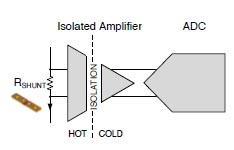
\includegraphics[width=\linewidth]{../assets/R-Shunt_Isolated_Sensor.jpg}
			\caption{Sensado por Resistencia Shunt}
		\end{subfigure}
		\begin{subfigure}[b]{0.4\linewidth}
			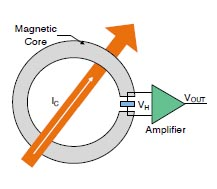
\includegraphics[width=\linewidth]{../assets/Open-loop_Hall_Sensor.jpg}
			\caption{Sensado por efecto Hall de loop abierto}
		\end{subfigure}
		\caption{Diagramas - Métodos de sensado de corriente}
		\label{fig:SenseMetods}
	\end{figure}
    
    \clearpage

	\subsubsection{Tecnología Seleccionada}
	
	Frente a los requerimientos y la naturaleza de un BMS hemos seleccionado 
    la tecnología de sensado de corriente por resistencia Shunt. 
    Actualmente existen en el mercado un sin número de soluciones de 
    amplificadores y moduladores aislados que permiten alcanzar precisas 
    mediciones de corrientes con este método logrando minimizar las inherencias 
    del entorno siempre y cuando se seleccione una resistencia Shunt adecuada.
	
	\noindent Las ventajas de la medición a partir del método de resistencia 
    shunt son:
	
	\begin{itemize}
		\item Bajo offset y baja susceptibilidad frente a influencias de campos 
            magnéticos externos y variaciones de temperatura.
		\item Alta linealidad de la solución en todo el rango de voltaje en 
            comparación a la solución basada en tecnología Hall, sobre todo en 
            la zona cercana a cero y la de saturación del nucleo. 
		\item Mejor resolución para mediciones de corriente continua frente a 
            las soluciones basadas en mediciones de efecto Hall. 
            Particularmente debido a la baja sensitividad que presenta frente a 
            las influencias de los campos magnéticos externos.
		\item Pueden soportar operaciones en ambientes de altas temperaturas 
            manteniendo la linealidad debido a su bajo TCR. 
            Los sensores de efecto Hall encuentran su rango de operación 
            fuertemente acotado.
		\item Facilidad que presenta la tecnología para la integración en 
            circuitos impresos priorizando el tamaño reducido.
		\item Disponibilidad en distribuidores nacionales
	\end{itemize}
	
	\noindent El integrado propuesto para el sensado de corriente es el INA226 
    de Texas Instruments. El INA226 es un conversor analógico digital de 16 bits 
    (ADC) que implementa una interfaz compatible I2C para la comunicación con el 
    módulo del control. El dispositivo monitorea simultaneamente la tensión que 
    cae en una resistencia shunt y la del bus de alimentación. Permite múltiples 
    calibraciones y seteos, entre ellos variar los tiempos de conversión y 
    definir conversiones múltiples que al implementar internamente un 
    multiplicador y divisor permite obtener lecturas directas de tensión y 
    potencia en amperes y en Vatios.
	
	Observamos en la Figura \ref{fig:ina226-commonimplementation} su 
    implementación modelo. 
	
	\begin{figure}[h!]
		\begin{center}
			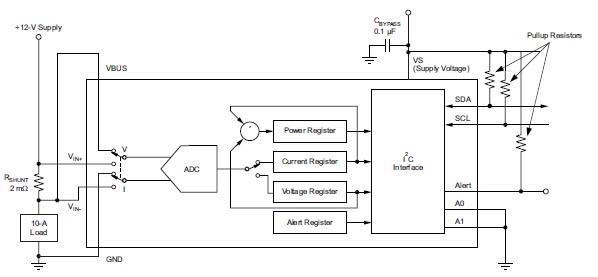
\includegraphics[width=0.6\linewidth]{assets/INA226-Common_Implementation}
			\caption{Implementación Tipo - INA226}
			\label{fig:ina226-commonimplementation}
		\end{center}	
	\end{figure}
	
    \clearpage	
	
	\subsection{Algoritmos de Estimación del Estado de Carga}

	La estimación del estado de carga es una de las tareas fundamentales dentro 
    del sistema de Administración de baterías ya que en base a esta información 
    se toman importantes decisiones, de ella dependen la optima ecualización de 
    carga de las celdas, no exceder los límites de Zona de Operación segura, 
    realizar acciones preventivas en caso del agotamiento de carga como ser 
    iniciar un apagado de seguridad y por último reportar al usuario la carga 
    restante en el pack.

	\noindent A priori hay 2 métodos básicos de estimación de carga, 
    el primero aprovecha la relación entre el SoC y el voltaje de circuito
    abierto u OCV (del ingles \emph{Open Circuit Voltage}) este método es 
    económico pero tiene 2 principales desventajas, la curva OCV vs SoC tiene 
    una región en la cual tiene valores de pendiente despreciable lo que genera 
    que entre el 80\% de carga y el 35\% aproximadamente, haya solo unas pocas 
    decenas de milivoltios de diferencia. Debido a esto un error de pocos 
    milivolts genera grandes diferencias en la estimación de la carga real. 
    Por otro lado la estimación mediante voltaje tiene problemas a la hora de 
    determinar el voltaje online, es decir cuando la batería esta conectada a 
    una carga las corrientes que circulan por el pack generan caidas de tensión 
    debido a las impedancias internas del pack, si estas no son tenidas en 
    cuenta pueden llevar a que el ecualizador del pack desbalancee aún más el 
    pack.

	\noindent El segundo método es el \textbf{\emph{Conteo de carga}} o 
    \textbf{\emph{Coulomb Counting}}, el mismo consiste en integrar la corriente 
    a lo largo del tiempo obteniendo así la carga total en el pack o SoC 
    mediante la ecuación \ref{SoC_Coulomb_C}, donde \emph{i} corresponde a la 
    corriente de la batería y $C_\eta$ la capacidad nominal de la misma.
	
	\begin{figure}[h!]
		\begin{center}
			\begin{equation}
				SoC=1-\frac{\int{i.dt}}{C_\eta}\label{SoC_Coulomb_C}
			\end{equation}	
		\end{center}
	\end{figure}
	
	\noindent Este método funciona muy bien en la zona donde el primer método 
    falla, sin embargo como todo proceso de integración, genera errores 
    iterativos en cada ciclo de cálculo generando que a lo largo del tiempo el 
    error absoluto de este método tienda a crecer.Además de la necesidad de 
    establecer un valor inicial de carga, estos puntos de referencia pueden ser 
    la carga total de la batería o la máxima DOD de manera que exigen a la 
    batería llegar a puntos límites de carga disminuyendo su vida útil.
	
	\noindent Debido a que nos interesa saber el SoC cuando la batería esta 
    entregando energía o siendo cargada se deben tener en cuenta los principales 
    factores que afectan a la estimación de carga on-line. Un modelo utilizado 
    para relacionar la tensión entre los bornes de la batería y el OCV utilizado 
    con gran frecuencia es el modelo eléctrico bosquejado en la 
    \emph{Fig. \ref{Electric_model}}, este modelo es coherente con el hecho de 
    que la tensión en los bornes de la batería en reposo es igual al OCV. 
    Pero al ser circulada por una corriente se deben tener en cuenta los 
    fenómenos dinámicos y la perdida por resistencias internas así como la 
    corriente de pérdida (auto descarga) de la batería.
	
	\begin{figure}[ht]
		\begin{center}
			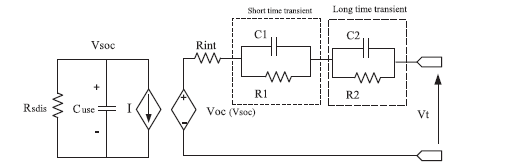
\includegraphics[width=0.7\textwidth]{electric_battery_model_2_order.png}
			\caption{Modelo Electrico de segundo orden con corriente de perdida.}
			\label{Electric_model}
		\end{center}
	\end{figure}

	\noindent Dada la naturaleza química de la batería, si se entra en detalle 
    se puede observar que los componentes que modelan la batería tienen un 
    comportamiento no lineal dependiendo del SoC y más aún se ven afectados por 
    el efecto de envejecimiento de las celdas, es decir, estamos es un sistema 
    no lineal no estacionario.

	\clearpage

	\noindent Como soluciones parciales fueron desarrollados varios métodos los 
    cuales son una solución de compromiso entre aproximaciones lo suficientemente 
    conservadoras para obtener el menor error posible y un alto costo 
    computacional cuyas exigencias de hardware elevan el costo y el espacio 
    necesario para su implementación, clasificándose según \cite{Hannan2017} 
    los siguientes métodos como convencionales:
	% \cite{Hannan2017}
	%A review of lithium-ion battery state of charge estimation and management
	%system in electric vehicle applications: Challenges and recommendations
	%M.A. Hannan,⁎, M.S.H. Lipu, A. Hussain, A. Mohamed 
	%el archivo se llama Lithium_SoC en la carpeta de papers

	\begin{itemize}
		\item Fuerza Electro-Motriz
		\item Estimación basada en modelos (Térmico y electroquímicos)
		\item Resistencia interna
		\item Espectroscopia Dieléctrica
	\end{itemize}
	
	\noindent Un gran avance en la estimación del estado de carga fue la 
    aplicación del filtro de Kalman para disminuir el error. 
    Esta es una herramienta estadística de análisis en espacio de estado que 
    mediante las matrices de varianza y covarianza estiman un vector de 
    soluciones con mayor precisión.
	Los Filtros de Kalman ven afectado su rendimiento a la hora de trabajar con 
    sistemas fuertemente no lineales, debido a esto surgen las variantes del 
    filtro de kalman extendido o EKF (del ingles \emph{Extended Kalman Filter}), 
    tipo \emph{unscented} o UKF (del ingles \emph{Unscented Kalman Filter}) y 
    tipo \emph{Sigma-point} o SPKF (del ingles \emph{Sigma-Point Kalman Filter}) 
    .\\
	
	\subsubsection{Método de estimación por FEM}

	Teniendo en cuenta la limitación del método de OCV para la estimación 
    mientras la batería esta siendo cargada o descargada, surge como solución 
    a esta problemática la estimación del OCV mediante el estudio de la 
    respuesta temporal de la tensión entre los terminales de la batería dado 
    su comportamiento temporal regido por una ecuación diferencial de primer 
    orden como se muestra en \emph{\ref{1er_orden_eq}}, siendo k una constante, 
    cuya solución es de la forma \emph{\ref{1er_orden_sol}}, lo cual se 
    corresponde con la gráfica de la \emph{Fig.\ref{EMF_Method}}.
	
	\begin{figure}[h!]
		\begin{center}
			\begin{equation}
				\frac{df(x)}{dx} = \alpha f(x)
				\label{1er_orden_eq}
			\end{equation}	
		\end{center}
	\end{figure}
	
	\begin{figure}[h!]
		\begin{center}
			\begin{equation}
				f(x)= x_{(\infty)}+(x_0-x_{(\infty)})e^{-\alpha x}
				\label{1er_orden_sol}
			\end{equation}	
		\end{center}
	\end{figure}
	
	\begin{figure}[h!]
		\begin{center}
			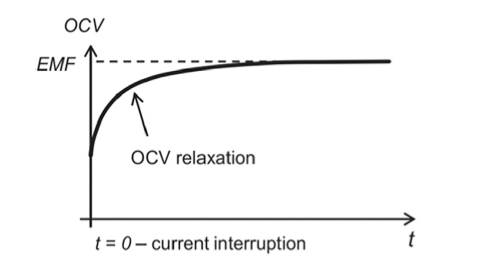
\includegraphics[width=0.7\textwidth]{EMF_Relaxation.png}
			\caption{Curva de relajación de una Batería de Li-Ion}
			\label{EMF_Method}
		\end{center}
	\end{figure}
	
	
	\clearpage
	
	\subsubsection{Estimación basada en modelos matematicos}

	Este método requiere un profundo conocimiento de los fenomenos físicos y 
    electroquímicos dentro de las baterías, como por ejemplo la concentración 
    de electrolito, concentración de material, densidad microscópica de corriente. 
    Esto constituye su principal desventaja ya que es complejo y la obtención 
    de parámetros no es trivial para todo tipo de baterías.
	
	Las celdas de Li-Ion se componen de 5 regiones: un electrodo negativo 
    colector de corriente, un electrodo compuesto poroso de inserción negativo, 
    un separador poroso, un electrodo compuesto poroso de inserción positivo y 
    un electrodo positivo colector de corriente. Esto en conjunto con las 
    ecuaciones \ref{Chrg_cons_hom_sol} - \ref{Butler_Volmer_kinetics} se detalla 
    en \cite{Li2016}.
	
	%\cite{Li2016}
	%Li-ion dynamics and state of charge estimation
	%Mingheng Li
	%Department of Chemical and Materials Engineering, California State Polytechnic University, Pomona, CA 91768, United States
	%el pdf se llama Li2016.pdf en la carpeta xxxx\bms\docs\Bibliography\Papers\SoC Papers
	
	\noindent Tomando como modelo un modelo unidimensional a lo largo de la 
    sección de la batería se aplican las siguentes ecuaciónes:
	
	\noindent Conservación de carga en un sólido homogéneo:

	\begin{figure}[h!]
		\begin{center}
			\begin{equation}
				\nabla \cdot (-\sigma\nabla\upvarphi_s)=-j^{Li} 
				\label{Chrg_cons_hom_sol}
			\end{equation}	
		\end{center}
	\end{figure}
	
	\noindent Conservación de masa en un sólido homogéneo:
	
	\begin{figure}[h!]
		\begin{center}
			\begin{equation}
				\frac{\partial c_s}{\partial t}=\nabla \cdot (D_s\nabla c_s) 
				\label{Mass_cons_hom_sol}
			\end{equation}	
		\end{center}
	\end{figure}
	
	\noindent Conservación de masa en un electrolito homogéneo:
	
	\begin{figure}[h!]
		\begin{center}
			\begin{equation}
				\varepsilon_e\frac{\partial c_e}{\partial t} + \nabla \cdot (-D_e\nabla c_e) = (\frac{1-t_+^0}{F})j^{Li}
				\label{Mass_cons_hom_electrolyte}
			\end{equation}	
		\end{center}
	\end{figure}
	
	\noindent Conservación de carga en un electrolito homogéneo:
	
	\begin{figure}[h!]
		\begin{center}
			\begin{equation}
				\nabla \cdot (\upkappa \nabla \upvarphi_e + \upkappa_D \nabla \ln c_e) = -j^{Li}
				\label{Chrg_cons_hom_electrolyte}
			\end{equation}	
		\end{center}
	\end{figure}
	
	\noindent Ecuación de Butler-Volmer de movimiento de cargas en una unión 
    entre un sólido conductor y una solución de Iones de Litio con el efecto de 
    doble capa eléctrica.
	
	\begin{figure}[h!]
		\begin{center}
			\begin{equation}
				j^{Li} = a_si_0[{e^\frac{F\eta}{2RT}-e^{-\frac{F\eta}{2RT}}}]+ a_sC_{dl}\frac{\partial{(\upvarphi_s - \upvarphi_e)}}{\partial t}
				\label{Butler_Volmer_kinetics}
			\end{equation}	
		\end{center}
	\end{figure}
	
	En las ecuaciones \ref{Chrg_cons_hom_sol} - \ref{Butler_Volmer_kinetics}, 
    $\mathrm{\sigma}$  conductividad de la fase sólida, $\mathrm{\upvarphi_s}$ 
    el potencial eléctrico de la fase sólida, $\mathrm{\upvarphi_e}$ el 
    potencial eléctrico del electrolito, $\mathrm{j^{Li}}$ la corriente 
    producida por el consumo de Li, t es el tiempo, c concentración de Iones de 
    Litio, D el coeficiente de difusión, F la constante de Faraday,
    $\mathrm{\varepsilon}$ es la fracción por volumen,
    $\mathrm{t_+^0}$ el número de transferencia, $\mathrm{\upkappa}$ la 
    conductividad del electrolito $\mathrm{\upkappa_D}$ la conductividad de la 
    difusión, $\mathrm{i_0}$ la densidad de corriente de intercambio, 
    $\mathrm{\eta}$ la sobretensión, a el area específica y $\mathrm{C_{dl}}$ 
    la capacidad de la doble capa. El subíndice s corresponde a la fase sólida y 
    e corresponde con el electrolito. 
    También teniendo en cuenta la relación de Bruggerman.
    % incompleto? 

    \clearpage

	\subsubsection{Estimación por resistencia interna}
	
	Este método utiliza el voltage y la corriente de la batería en 
    conjunto para determinar la resistencia interna. La metodologia de este
    metodo consiste en excitar a la bateria con pulsos de corrientes lo
    suficientemente breves como para que la variacion de tension sea
    completamente atribuida a la resistencia interna y no al efecto quimico de
    carga/descarga de ella, como resultado, la resistencia interna se puede
    calcular aplicando la ley de Ohm.
	
	\begin{figure}[h!]
		\begin{center}
			\begin{equation}
				\frac{\Delta V}{\Delta I} = R_\Omega 
				\label{Internal_resistance_EQ}
			\end{equation}	
		\end{center}
	\end{figure}
	
	\noindent Teniendo en cuenta que si el período del pulso es mayor, 
    la medición acumula un error considerablemente mayor respecto a pulsos breves 
    y teniendo en cuenta que este método tiene una gran precisión únicamente en 
    valores de SoC cercanos a la descarga, debido a que varia mucho en este rango, 
    y al bajo valor de las resistencias (del orden de los miliohmios) como se 
    puede observar en la Figura \ref{Internal_resistance}, 
    extraida de \cite{hentunen2014}, este método no resulta atractivo debido a 
    las dificultades para obtener valores precisos de SoC, logrando que sea
    dificil de implementar en BMS destinados a operaciones criticas.
	
	%\cite{hentunen2014}
	%Time-Domain Parameter Extraction Method for
	%Thevenin-Equivalent Circuit Battery Models
	%Ari Hentunen, Member, IEEE, Teemu %Lehmuspelto, Member, IEEE, and Jussi Suomela
	%el pdf se llama hentunen2014 en la carpeta xxxx\bms\docs\Bibliography\Papers\SoC Papers

	\begin{figure}[h!]
		\begin{center}
			\includegraphics[width=0.7\textwidth]{Ro_vs_SoC.png}
			\caption{Resistencia en Corriente continua de una batería de Li-Ion 
                     vs. SoC obtenida por HPPC}
			\label{Internal_resistance}
		\end{center}
	\end{figure}

	\clearpage

	\subsubsection{Espectroscopía Dieléctrica (EIS)}

	Este estudio consiste en llevar a la celda a un estado de carga conocido, 
    y luego de un período de relajación se excita los terminales con una onda 
    senoidal de tensión o corriente y se mide la respuesta de la misma. 
    En la Figura \ref{EIS_Nyquist} se observan las curvas obtenidas por 
    Mingheng Li (referenciar!!) basadas en un modelo físico basado en los 
    principios de conservación de masa y carga en una interfaz entre un sólido 
    y un electrolito detallado en \cite{Li2016}, para distintos estados de carga 
    y en un amplio rango de frecuencias. 
	
	\begin{figure}[h!]
		\begin{center}
			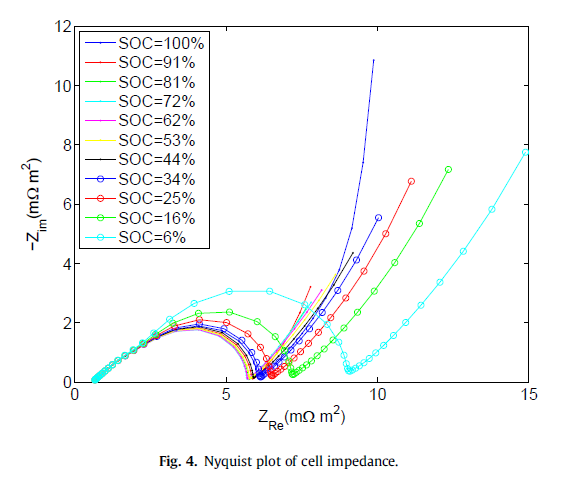
\includegraphics[width=0.7\textwidth]{EIS_Nyquist.png}
			\caption{Diagrama de Nyquist - Espectroscopía Dieléctrica (EIS) de 
                     una batería de Li-Ion obtenida por barrido frecuencial.}
			\label{EIS_Nyquist}
		\end{center}
	\end{figure}
	
	\clearpage
	
	\subsection{Filtros de Kalman}

	Este tipo de filtros toma importancia en sistemas de naturaleza estocástica. 
    Cuya dinámica es afectada por ruido cuya distribución de probabilidad es 
    de caracter \emph{Gaussiano} o normal. Este es un algoritmo recursivo que 
    corrige las estimaciones mediante la probabilidad conjunta de una o varias 
    mediciones de un fenómeno y su estimación obtenida por modelos matemáticos 
    generados en base al conocimiento del sistema.
	
	\noindent Dado un sistema lineal cuya dinámica es descripta por las 
    siguientes ecuaciones:
	
	\begin{figure}[h!]
		\begin{center}
			\begin{equation}
				x_{k+1}= Ax_{k} + w_{k}
				\label{KF_equation01}
			\end{equation}	
		\end{center}
	\end{figure}
	
    \noindent Donde $\mathrm{x_{k}}$ es el vector de estados en el instante de 
    tiempo k, A es la matriz de transición de estados y $\mathrm{w_{k}}$ ruido 
    aditivo gaussiano asociado al modelo del proceso con matriz de varianza Q. 
    Además podemos expresar el vector de observación o medición $\mathrm{z_{k}}$ 
    de los estados $\mathrm{x_{k}}$ como:
	
	\begin{figure}[h!]
		\begin{center}
			\begin{equation}
				z_{k}= Hx_{k} + v_{k}
				\label{KF_equation02}
			\end{equation}	
		\end{center}
	\end{figure}
	
	\noindent Donde H es la matriz de conexión entre los estados y las 
    observaciones sin ruido, es decir que mediciones se están tomando y que 
    estado representan. Por el otro lado $\mathrm{v_{k}}$ es el ruido aditivo 
    gaussiano asociado a la medición con matriz de varianza R.
	
	\noindent Definiendo la función de costo al error cuadrático medio en la 
    estimación de $\mathrm{x_k}$ (falta definicion aca)
	
	\noindent Definiendo al error como: 
	
	\begin{figure}[h!]
		\begin{center}
			\begin{equation}
				e_{k} = x_k  - \hat{x}_k
				\label{KF_error}
			\end{equation}	
		\end{center}
	\end{figure}
	
	\noindent De manera que podemos expresar la matriz de covarianza del error 
    en el instante k como:
	
	\begin{figure}[h!]
		\begin{center}
			\begin{equation}
				P_{k} = E[e_k.{e_k}^{T}] = E[(x_k-\hat{x}_k).(x_k-\hat{x}_k)^{T}]
				\label{KF_equation03}
			\end{equation}	
		\end{center}
	\end{figure}
	
    \noindent Podemos expresar $\mathrm{\hat{x}_k}$ como: 
	
	\begin{figure}[h!]
		\begin{center}
			\begin{equation}
				\hat{x}_k = \hat{x}^\prime_k + K_k (z_k - H\hat{x}^\prime_k)
				\label{KF_equation04}
			\end{equation}	
		\end{center}
	\end{figure}
	
    \noindent Donde $\mathrm{K_k}$ es la ganancia de Kalman la cual pondera 
    según el criterio de minimización del error cuadrático medio si
    $\mathrm{\hat{x}_k}$ es próxima a $\mathrm{\hat{x}^\prime_k}$ o al vector 
    $\mathrm{z_k}$.
	
    \noindent Si reemplazamos $\noindent{z_k}$ en la ecuación 
    \ref{KF_equation04} por la expresión \ref{KF_equation02} se obtiene la 
    expresión del error de la estimación a priori $\mathrm{\hat{x}^\prime_k}$ 
    detallada a continuación:
	
	\begin{figure}[h!]
		\begin{center}
			\begin{equation}
				\hat{x}_k = \hat{x}^\prime_k + K_k (Hx_{k} + v_{k} - H\hat{x}^\prime_k)
				\label{KF_equation05}
			\end{equation}	
		\end{center}
	\end{figure}

    \clearpage
	
	\noindent Reacomodando los terminos, 
	
	\begin{figure}[h!]
		\begin{center}
			\begin{equation}
				\hat{x}_k = \hat{x}^\prime_k + K_k H (x_{k}  - \hat{x}^\prime_k) + K_kv_{k}
				\label{KF_equation06}
			\end{equation}	
		\end{center}
	\end{figure}
	
	\noindent Multiplicando por (-1) y luego sumando en ambos miembros de la 
    ecuación \ref{KF_equation06} el termino $\noindent{x_k}$ 
	
	\begin{figure}[h!]
		\begin{center}
			\begin{equation}
				x_k - \hat{x}_k = x_{k} -\hat{x}^\prime_k - K_k H (x_{k}  - \hat{x}^\prime_k) - K_kv_{k}
				\label{KF_equation08}
			\end{equation}	
		\end{center}
	\end{figure}
	
	\begin{figure}[h!]
		\begin{center}
			\begin{equation}
				x_k - \hat{x}_k = (I-K_k H)(x_k - \hat{x}^\prime_k) - K_kv_{k}
				\label{KF_equation09}
			\end{equation}	
		\end{center}
	\end{figure}
	
	
	\noindent Reemplazando luego en la ecuación \ref{KF_equation03} la expresión 
    $\noindent{x_k - \hat{x}_k}$ por el de la ecuación \ref{KF_equation09} 
    obtenemos la expresión de $\mathrm{P_k}$ como función del error de la 
    estimación a priori:
	
	\begin{figure}[h!]
		\begin{center}
			\begin{equation}
				P_k = E[[(I-K_k H)(x_k - \hat{x}^\prime_k) - K_kv_{k}][ (I-K_k H)(x_k - \hat{x}^\prime_k) - K_kv_{k}]^T]
				\label{KF_equation10}
			\end{equation}	
		\end{center}
	\end{figure}
	
	\noindent Aplicando propiedades de la transpuesta de una matriz e ignorando 
    los terminos relativos a la correlación entre el ruido de la medición y el 
    error de la estimación a priori:
	
	\begin{figure}[h!]
		\begin{center}
			\begin{equation}
				P_k = E[[(I-K_k H)(x_k - \hat{x}^\prime_k)(x_k - \hat{x}^\prime_k)^T(I-K_k H)^T + K_k v_{k} v_{k}^T K_k^T 
				\label{KF_equation11}
			\end{equation}	
		\end{center}
	\end{figure}
	
	\noindent Teniendo en cuenta que la esperanza de una matriz, que no es 
    variable aleatoria, es la misma matriz:
	
	\begin{figure}[h!]
		\begin{center}
			\begin{equation}
				P_k = (I-K_k H) E[(x_k - \hat{x}^\prime_k)(x_k - \hat{x}^\prime_k)^T](I-K_k H)^T + K_k E[v_{k} v_{k}^T] K_k^T 
				\label{KF_equation12}
			\end{equation}	
		\end{center}
	\end{figure}
	
	\noindent Obteniendose así la expresión de la ecuación de actualización de 
    la matriz de covarianza:
	
	\begin{figure}[h!]
		\begin{center}
			\begin{equation}
				P_k = (I-K_k H)P^\prime_k(I-K_k H)^T + K_k R K_k^T 
				\label{KF_equation13}
			\end{equation}	
		\end{center}
	\end{figure}
	
	\clearpage
	
    \noindent Recordando la forma de la matriz $\mathrm{P_k}$ y observando que 
    su traza, definida como la sumatoria de todos los elementos de la diagonal 
    principal, es la suma del error cuadrático medio o MSE (del ingles
    \emph{Mean Square Error}), de manera que podemos afirmar que minimizandola 
    podemos minimizar el MSE.

	\begin{equation}
		P_k = 
		\begin{bmatrix}
			e_{1k}e_{1k} & e_{1k}e_{2k} &	\dots  & e_{1k}e_{nk} \\
			e_{2k}e_{1k} & e_{2k}e_{2k} &	\dots  & e_{2k}e_{nk} \\
			\vdots       &   \vdots     &	\ddots & \vdots       \\
			e_{nk}e_{1k} & e_{nk}e_{2k} &	\dots  & e_{nk}e_{nk} \\
		\end{bmatrix}
	\end{equation}
	
    \noindent De manera que buscamos $\mathrm{K_k}$ que cumpla con este 
    requisito, para lo cual haremos la expansión de la ecuación 
    \ref{KF_equation13} para obtener luego una expresión de la traza.
	
	\begin{figure}[h!]
		\begin{center}
			\begin{equation}
				P_k = P^\prime_k - K_k H P^\prime_k - P^\prime_k H^T K^T_k + K_k (H P^\prime_k H^T + R) K^T_k
				\label{KF_equation14}
			\end{equation}	
		\end{center}
	\end{figure}
	
    \noindent Siendo la expresión de $\mathrm{T[P_k]}$
	
	\begin{figure}[h!]
		\begin{center}
			\begin{equation}
				T[P_k] = T[P^\prime_k] - T[K_k H P^\prime_k] - T[P^\prime_k H^T K^T_k] + T[K_k (H P^\prime_k H^T + R) K^T_k]
				\label{KF_equation15}
			\end{equation}	
		\end{center}
	\end{figure}
	
    \noindent Ya que $\mathrm{P^\prime_k}$ es simétrica y que la traza de una 
    matriz es igual a la traza de su transpuesta.
	
	\begin{figure}[h!]
		\begin{center}
			\begin{equation}
				P^{\prime T}_k  = P^\prime_k
				\label{KF_equation16}
			\end{equation}	
		\end{center}
	\end{figure}
	
	\noindent Podemos escribir
	
	\begin{figure}[h!]
		\begin{center}
			\begin{equation}
				P^\prime_k H^T K^T_k = P^{\prime T}_k H^T K^T_k = (K_k H P^\prime_k )^T
				\label{KF_equation17}
			\end{equation}	
		\end{center}
	\end{figure}
	
	\begin{figure}[h!]
		\begin{center}
			\begin{equation}
				T[P^\prime_k H^T K^T_k] = T[K_k H P^\prime_k]
				\label{KF_equation18}
			\end{equation}	
		\end{center}
	\end{figure}
	
	\noindent Reemplazando \ref{KF_equation18} en \ref{KF_equation15},

	\begin{figure}[h!]
		\begin{center}
			\begin{equation}
				T[P_k] = T[P^\prime_k] -2 T[K_k H P^\prime_k] + T[K_k (H P^\prime_k H^T + R) K^T_k]
				\label{KF_equation19}
			\end{equation}	
		\end{center}
	\end{figure}
	
	\noindent Para obtener el valor mínimo calculamos la derivada de 
    $\mathrm{T[P_k]}$ respecto a $\mathrm{K_k}$
	
	\begin{figure}[h!]
		\begin{center}
			\begin{equation}
				\frac{dT[P_k]}{dK_k} = -2 (H P^\prime_k)^T + 2K_k (H P^\prime_k H^T + R)
				\label{KF_equation20}
			\end{equation}	
		\end{center}
	\end{figure}
	
	\noindent Luego igualando la ecuación \ref{KF_equation20} a 0 y despejando 
    obtenemos la expresión de la Ganancia de Kalman ($\mathrm{K_k}$):
	
	\begin{figure}[h!]
		\begin{center}
			\begin{equation}
				K_k = (H P^\prime_k)^T (H P^\prime_k H^T + R)^{-1} 
				\label{KF_equation21}
			\end{equation}	
		\end{center}
	\end{figure}
	
	\clearpage
	
    \noindent Definiendo a $\mathrm{S_k}$ como:
	
	\begin{figure}[h!]
		\begin{center}
			\begin{equation}
				S_k = (H P^\prime_k H^T + R)
				\label{KF_equation22}
			\end{equation}	
		\end{center}
	\end{figure}
	
	\noindent La ecuación \ref{KF_equation21} queda:
	
	\begin{figure}[h!]
		\begin{center}
			\begin{equation}
				K_k = (H P^\prime_k)^T S_k^{-1} 
				\label{K_Gain}
			\end{equation}	
		\end{center}
	\end{figure}
	
    \noindent Reemplazando la expresión de $\mathrm{K_k}$ obtenido, en la 
    ecuación  \ref{KF_equation14}, se cancela el tercer término con el cuarto 
    término y queda:
	
	\begin{align}
		P_k  &= P^\prime_k + P^\prime_k H^T (H P^\prime_k H^T + R)^{-1} H P^\prime_k \nonumber \\
		P_k  &= P^\prime_k - K_k H P^\prime_k \nonumber\\
		P_k  &= (I - K_k H) P^\prime_k	
		\label{KF_equation23}	
	\end{align}
	
    \noindent La proyección del vector de estados $\mathrm{x_k}$ en el instante 
    $\mathrm{k+1}$ se obtiene como:
	
	\begin{figure}[h!]
		\begin{center}
			\begin{equation}
				\hat{x}^\prime_{k+1} = A \hat{x}_k 
				\label{x_k_projection}
			\end{equation}	
		\end{center}
	\end{figure}
	
    \noindent Para luego proyectar la matriz de covarianza de error
    $\mathrm{P_k}$ en el instante $\mathrm{k+1}$.
	
	\noindent Haciendo uso de la ecuación \ref{KF_equation03} y extendiéndola 
    para $\mathrm{e^\prime_{k+1}}$:
	
	\begin{figure}[h!]
		\begin{center}
			\begin{equation}
				P_{k+1} = E[e_{k+1}.e_{k+1}^{T}] = E[(A e_k-w_k).(A  e_k-w_k)^{T}]
				\label{projection_p_k_aux}
			\end{equation}	
		\end{center}
	\end{figure}
	
    \noindent Cabe destacar que el ruido del proceso $\mathrm{w_k}$ no tiene 
    correlación alguna respecto a $\mathrm{e_k}$ ya que el primero es el ruido 
    presente entre k y k+1 y $\mathrm{e_k}$ es el error resultante de todos los 
    calculos previos hasta el instante k.
	
	\begin{figure}[h!]
		\begin{center}
			\begin{equation}
				P^\prime_{k+1} = E[A e_{k}.e_{k}^{T}A^{T}]+ E[w_k w_k^{T}]= A P_k A^{T} + Q
				\label{projection_p_k}
			\end{equation}	
		\end{center}
	\end{figure}
	
	\clearpage
	
	\subsubsection{Filtro de Kalman: resumen}
	
	Como dijimos los filtros de Kalman son algoritmos recursivos, los mismos se 
    componen por las siguientes ecuaciones descriptas anteriormente:
	
	\begin{table}[h!]
		\centering
		\begin{tabular}{|c|c|}
			\hline
			\rule{0pt}{4ex}	Ganancia de Kalman 							& $K_k = (H P^\prime_k)^T S_k^{-1}$  \\ \hline
			\rule{0pt}{4ex}	Actualización de la estimación			    &  $\hat{x}_k = \hat{x}^\prime_k + K_k (z_k - H\hat{x}^\prime_k)$\\ \hline
			\rule{0pt}{4ex}	Actualización de la matriz de covarianza    & $P_k = (I - K_k H) P^\prime_k$ \\ \hline
			\multirow{2}{*}{Proyeccion en k+1}        		  			& \rule{0pt}{4ex} $\hat{x}^\prime_{k+1} = A \hat{x}_k$ \\ \cline{2-2}
			& \rule{0pt}{4ex} $P^\prime_{k+1} = A P_k A^{T} + Q$ \\ \hline
		\end{tabular}
		\label{Ecuaciones_Kalman}
	\end{table}
	
	
    \noindent Los filtros de Kalman pueden ser interpretados intuitivamente 
    partiendo de la base de que tenemos la medición antes definida como 
    $\mathrm{z_k}$ y corriendo en paralelo tenemos un modelo matemático 
    calculando el estado actual o vector de estados actual de nuestro sistema el 
    cual notaremos como $\mathrm{\hat{x}^\prime_k}$ y llamaremos estimación a 
    priori de $\mathrm{x_{t}}$.
	
	\noindent Ambos valores son afectados por ruido asociado, de manera que 
    podemos ponderar ambas de manera de obtener una medición más certera.
	
	\noindent Como se observa en la Figura \ref{KF_Integration_concept} en base 
    a las distribuciones de $\mathrm{z_k}$ y $\mathrm{\hat{x}^\prime_k}$ 
    obtenemos una nueva $\mathrm{\hat{x}_k}$ la cual tiene una menor varianza.
	
	\begin{figure}[h!]
		\begin{center}
			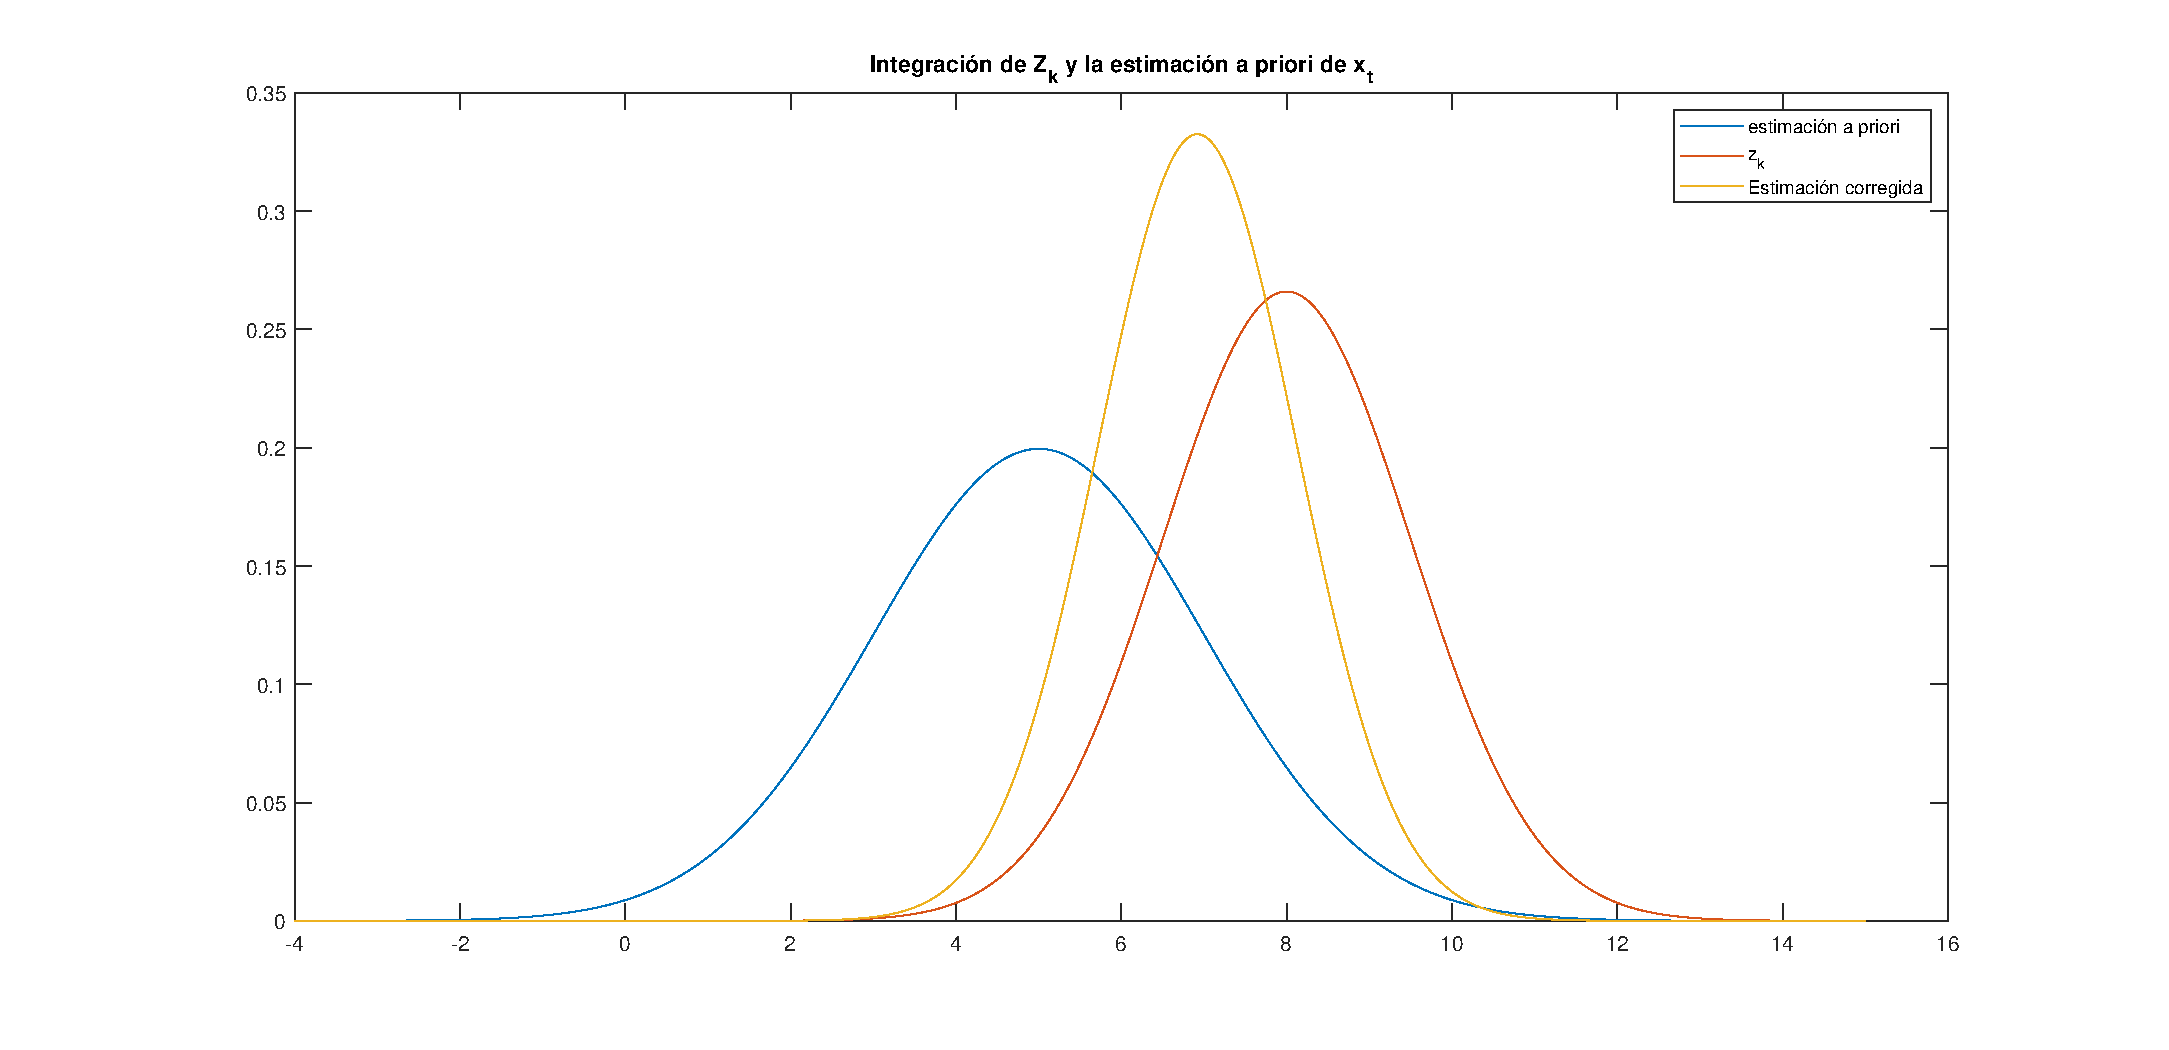
\includegraphics[width=1\textwidth]{KF_Integration_concept.eps}
			\caption{Gráfico ilustrativo de la estimación de $x_{t}$ mediante $z_k$ y $\hat{x}^\prime_k$ .}
			\label{KF_Integration_concept}
		\end{center}
	\end{figure}
	
	\clearpage
	
	\subsection{Simulaciones}

	\subsubsection{Filtro de Kalman}

	\noindent Para la implementación de este filtro es necesario obtener un 
    modelo en espacio de estados de la batería de la forma:
	
	\begin{align}
		\dot{x}(t) = Ax+Bu	\nonumber\\
		y(t)=Cx+Du
		\label{SS_Model_generic}	
	\end{align}
	
	
	\noindent Para tal fin tomamos como referencia un modelo eléctrico con 2 
    elementos RC en serie, también conocido como modelo de Randles de segundo 
    orden, representado en la figura \ref{Randles_2do}, ya que este módelo 
    tiene amplia aceptación debido a que ofrece un grado de ajuste alto sin 
    resultar en un excesivo costo computacional en comparación con modelos 
    electroquímicos de la batería.
	
	\begin{figure}[h!]
		\begin{minipage}[c]{0.45\textwidth}
			\centering
			\ctikzset{bipoles/length=1.0cm}
			\ctikzset{bipoles/resistor/height=.3}
			
			\begin{circuitikz}[american]
				
				
				\draw (0,0) to[R=$R_0$] (3,0) -- (3,-0.5) to[R=$R_1$] (6,-0.5) -- (6,0);
				\draw (3,0) -- (3,0.5) to[C=$C_1$,v=$ $] (6,0.5) -- (6,0);
				\draw (6,0) to[short,-*] (6.5,0) -- (7,0) -- (7,0.5) to[C=$C_2$,v=$ $] (10,0.5) to[short,-o] (10,0);
				\draw (7,0) -- (7,-0.5) to[R=$R_2$] (10,-0.5) -- (10,0) to[short,f=$i$] (11.5,0);
				\draw  (0,0) to[battery2=$OCV(SoC)$] (0,-3) -- (11.5,-3); 
				\draw  (11.5,0) to [open,v=$v$,invert] (11.5,-3);
				\draw (8.5,1.75) node[anchor=north]{$V_{C2}$};
				\draw (4.5,1.75) node[anchor=north]{$V_{C1}$};
			\end{circuitikz}
		\end{minipage}
		\caption{Circuito de Randles de segundo orden.}
		\label{Randles_2do}
	\end{figure}
	
	\noindent La fuente de tensión controlada $OCV(SoC)$ es linealizada para 
    obtener un modelo lineal de la batería e ignoramos el hecho de la histéresis 
    respecto a la carga y a la descarga.
	
	\noindent Obteniendo una ecuación lineal de la forma \ref{SoC_linearized}, 
    cuyos parametros fueron obtenidos mediante la función 
    \emph{polyfit} de matlab como se muestra en la figura \ref{SoC_vs_OCV}.
	
	\begin{figure}[h!]
		\begin{center}
			\begin{equation}
				OCV = SoC \times K_e + OCV_0
				\label{SoC_linearized}
			\end{equation}	
		\end{center}
	\end{figure}
	
	\clearpage
	
	\begin{figure}[h!]
		\begin{center}
			\includegraphics[width=1\textwidth]{SoC_vs_OCV.eps}
			\caption{Curva de SoC vs OCV con su correspondiente linealización }
			\label{SoC_vs_OCV}
		\end{center}
	\end{figure}
	
	\noindent Nuestro modelo eléctrico tiene 2 grados de libertad y se agrega 
    una $\mathrm{3^{er}}$ variable de estado que es el estado de carga de la 
    batería. Luego tomando la expresión diferencial de la ecuación 
    \ref{SoC_Coulomb_C}, seleccionando arbitrariamente las tensiones en 
    $C_1$ y $C_2$, y tomando como entrada del sistema la corriente de la 
    batería y como salida la tensión en bornes de la misma obtenemos el 
    siguiente conjunto de ecuaciones:
	
	\begin{equation}
		\begin{array}{llcllcl}
			\dot{x} & = & \begin{bmatrix}
				-\frac{1}{R_1 C_1} & 			0 		& 0 \\
				0				   & -\frac{1}{R_2 C_2} & 0 \\
				0      			   &   			0       & 0 \\
			\end{bmatrix} & x & + & 	\begin{bmatrix}
				-\frac{1}{R_1 C_1} \\
				-\frac{1}{R_2 C_2}  \\
				-\frac{1}{3600 S_{C,a}}\\
			\end{bmatrix} & i \\
			y & = & \begin{bmatrix}
				-1-1-K_e 
			\end{bmatrix} & x & + & \begin{bmatrix}
				R_0
			\end{bmatrix} & i \\
		\end{array}
	\end{equation}
	
    \noindent Donde $\mathrm{S_{C,a}}$ es la capacidad nominal en Ah de la 
    batería. 

    \noindent Para hacer un ajuste de parámetros de las baterías se utilizó un 
    dataset provisto por la universidad de Winsconsin-Madison por el 
    Dr. Phillip Kollmeyer \cite{Kollmeyer2018}. Si bien todos los parámetros 
    son dependientes del estado de carga, seleccionamos los correspondientes al 
    90\%, ya que las variaciones mas fuertes de los mismos se dan al entre el 
    0-10\% y en valores cercanos al 100\%.
	
	\begin{figure}[h!]
		\begin{center}
			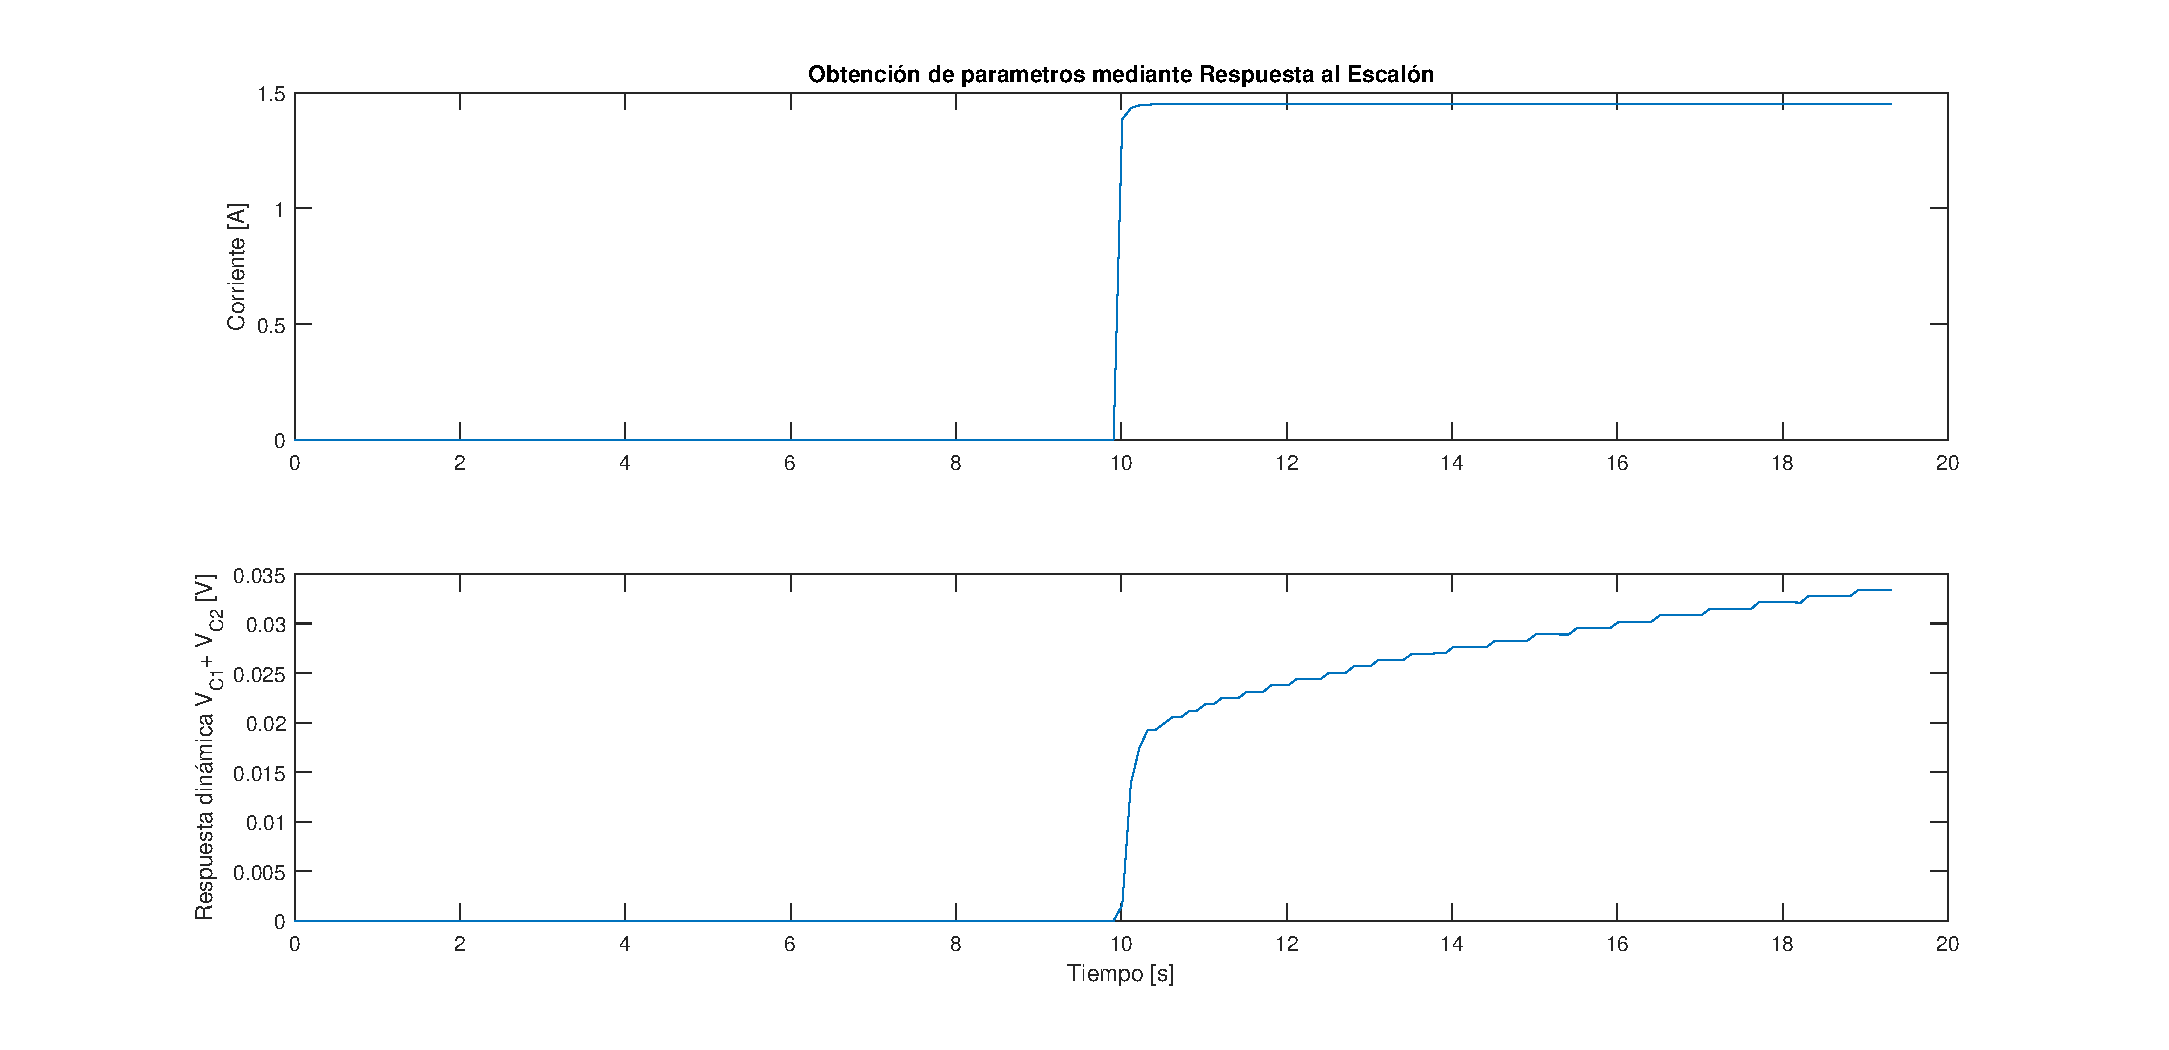
\includegraphics[width=0.85\textwidth]{rta_escalon.eps}
			\caption{Estudio de la Rta al escalón para estimación de parámetros}
			\label{rta_escalon}
		\end{center}
	\end{figure}
	
	\noindent También se necesita proporcionar valores de varianza del modelo, 
    ruido al que están sometidas las variables medibles, el estado inicial 
    estimado y la varianza de esta estimación denominadas Q, R, $\mathrm{x_0}$ 
    y $\mathrm{P_0}$ respectivamente.
	
	\noindent Partiendo de la base que nuestro sistema debe ser robusto ante la 
    mala estimación inicial del estado de carga vamos a proponer un vector de 
    estimación de estado inicial con un SoC con un error de 80\%.
	
	\begin{equation}
		\begin{array}{llll}
			P_0 & = & \begin{bmatrix}
				1 & 0 & 0 \\
				0 & 1 & 0 \\
				0 & 0 & 1 \\
			\end{bmatrix} 
		\end{array} \nonumber
	\end{equation}

    \noindent El ciclo de la bateria esseleccionado comienza con la batería 
    cargada al 100\%, por lo que un error del 80\% se corresponde con 0.2 en el 
    estado de carga relativo.

	\begin{equation}
		\begin{array}{llll}
			x_0 & = & \begin{bmatrix}
				0 \\
				0 \\
				0.2 \\
			\end{bmatrix} 
		\end{array} \nonumber
	\end{equation}

    \noindent El error en nuestra observación es del orden de los milivoltios
    (mV) calculado en base a la resolución del sensor.

	\begin{equation}
		R = 0.01  \nonumber
	\end{equation}
	
	\noindent El error en nuestro modelo se estima bajo ya que los dataset nos 
    proveen una buena fuente de información obtenida en base a ensayos de 
    laboratorio

	\begin{equation}
		\begin{array}{llll}
			Q & = & \begin{bmatrix}
				1\cdot10^{-6} & 0 & 0 \\
				0 & 1\cdot10^{-6} & 0 \\
				0 & 0 & 1\cdot10^{-6} \\
			\end{bmatrix} 
		\end{array} \nonumber
	\end{equation}
	
	\clearpage
	
	\noindent Por último se volcaron estos parámetros en un bloque de la 
    librería \emph{System Identification Toolbox} de MatLAB que corre el 
    algoritmo del filtro de Kalman. Además se simuló en paralelo el circuito 
    eléctrico equivalente, como se observa en la Figura \ref{simulink_diagram}.

	\begin{figure}[h!]
		\begin{center}
			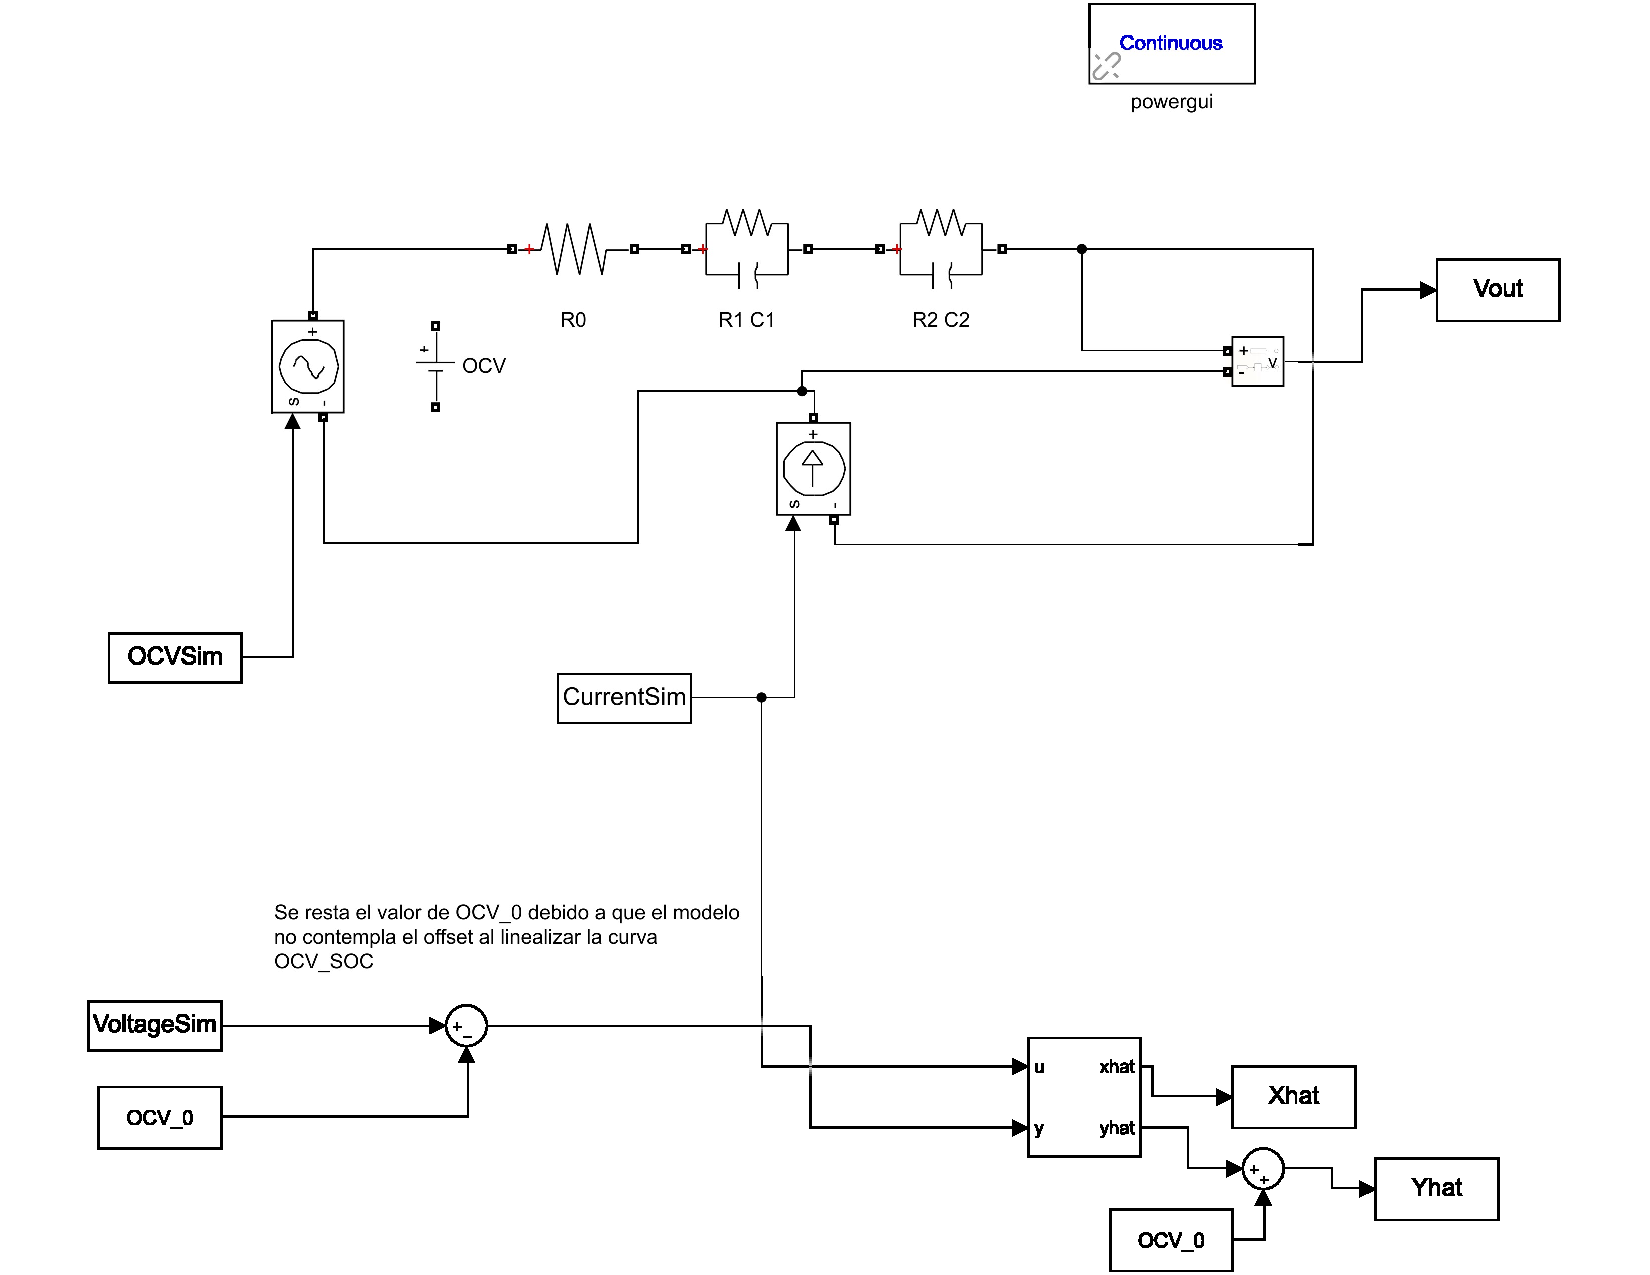
\includegraphics[width=1\textwidth]{simulink.pdf}
			\caption{Diagrama de Simulink utilizado para simular el Filtro de Kalman}
			\label{simulink_diagram}
		\end{center}
	\end{figure}
	
	\clearpage
	
	\noindent Los resultados de la simulación se muestran a continuación en las 
    Figuras \ref{Tension_sim} y \ref{Tension_sim_zoom} correspondientes a la 
    tensión en bornes de la batería y a las Figuras \ref{Drive_Cycle_1_SoC_sim} 
    y \ref{error_SOC_Sim}, las cuales corresponden al SoC simulado y a un 
    contraste del error tomando como valor verdadero el SoC provisto por el dataset.
	
	\begin{figure}[h!]
		\begin{center}
			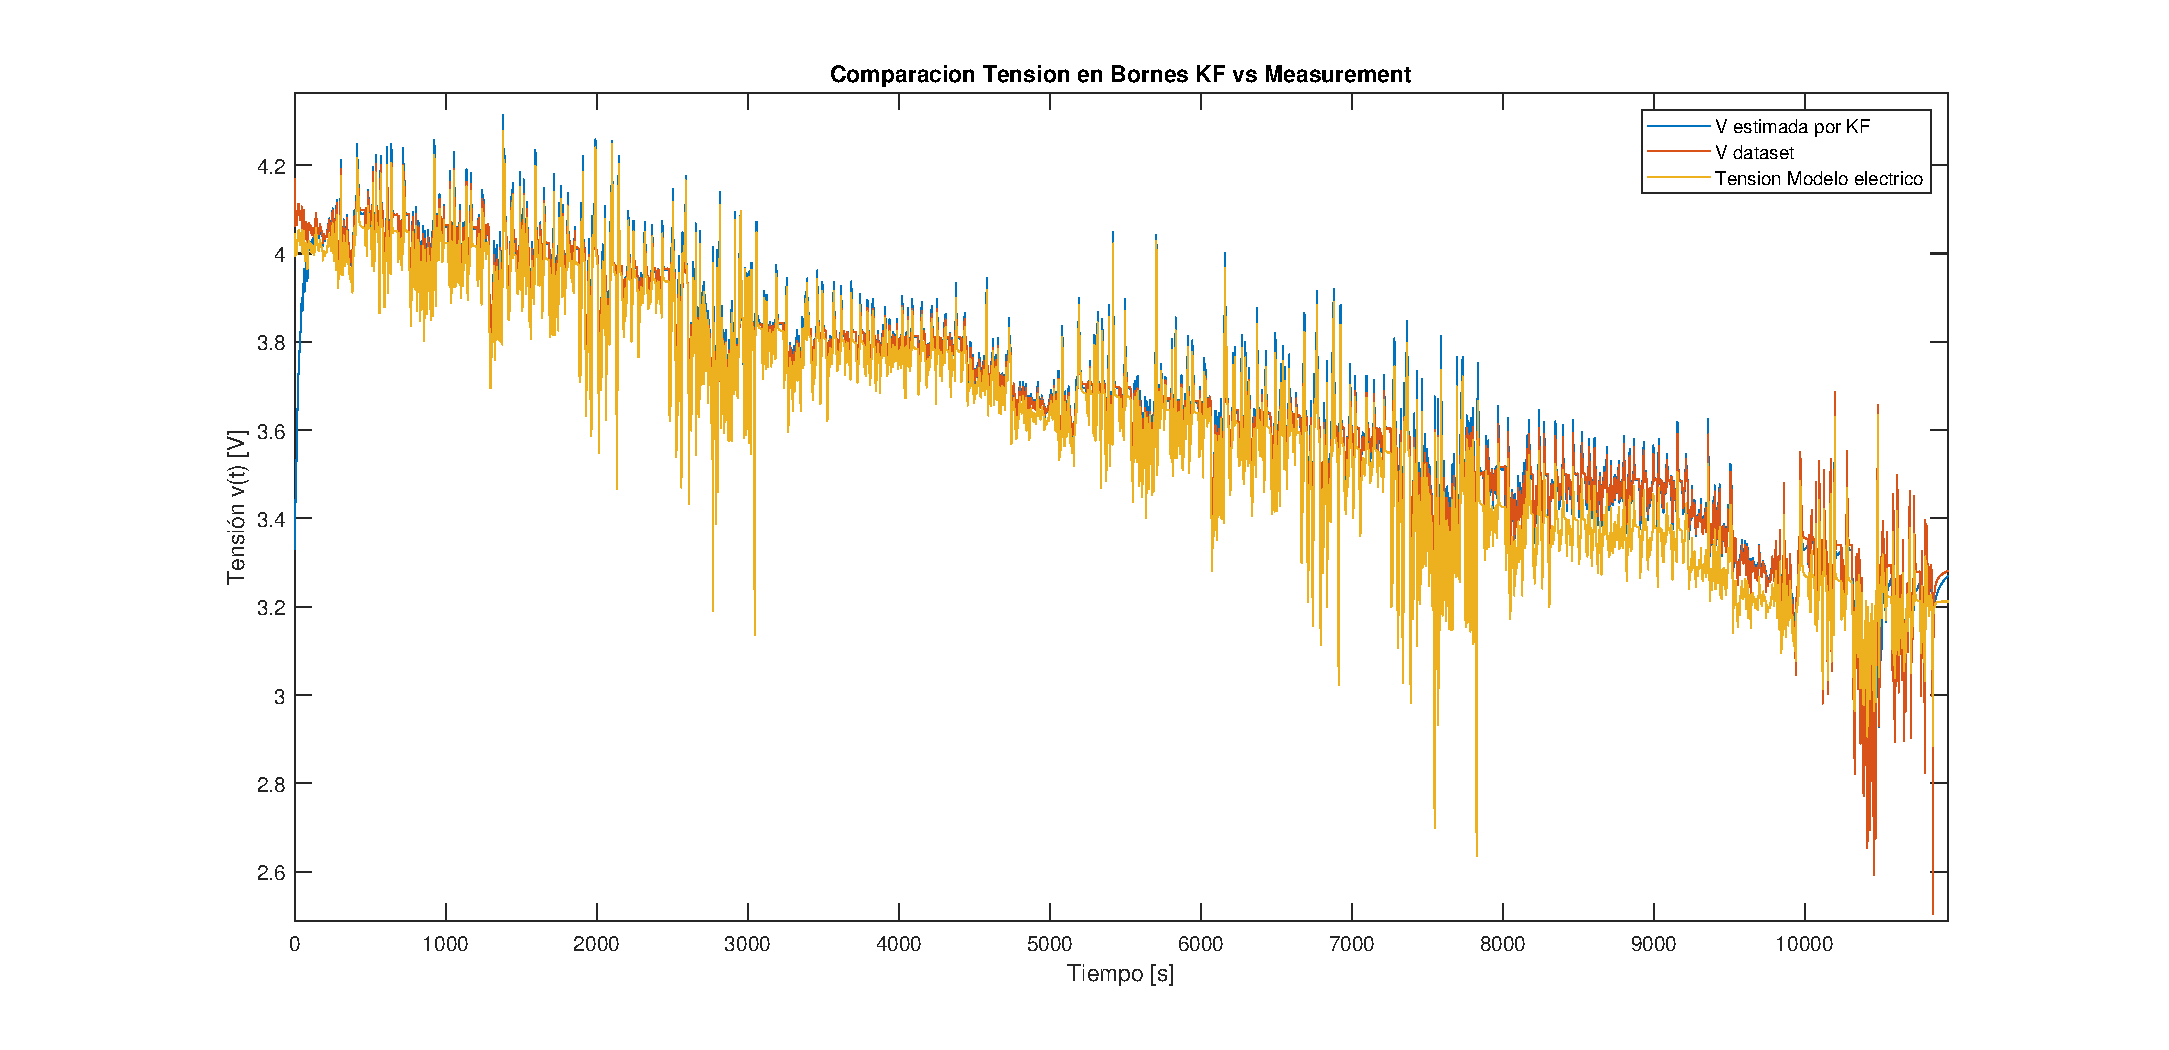
\includegraphics[width=1\textwidth]{Tension_Sim.eps}
			\caption{Resultado de la Simulación de la tensión en bornes de la 
                     batería sometida a condiciones de ciclo de manejo}
			\label{Tension_sim}
		\end{center}
	\end{figure}
	
	\begin{figure}[h!]
		\begin{center}
			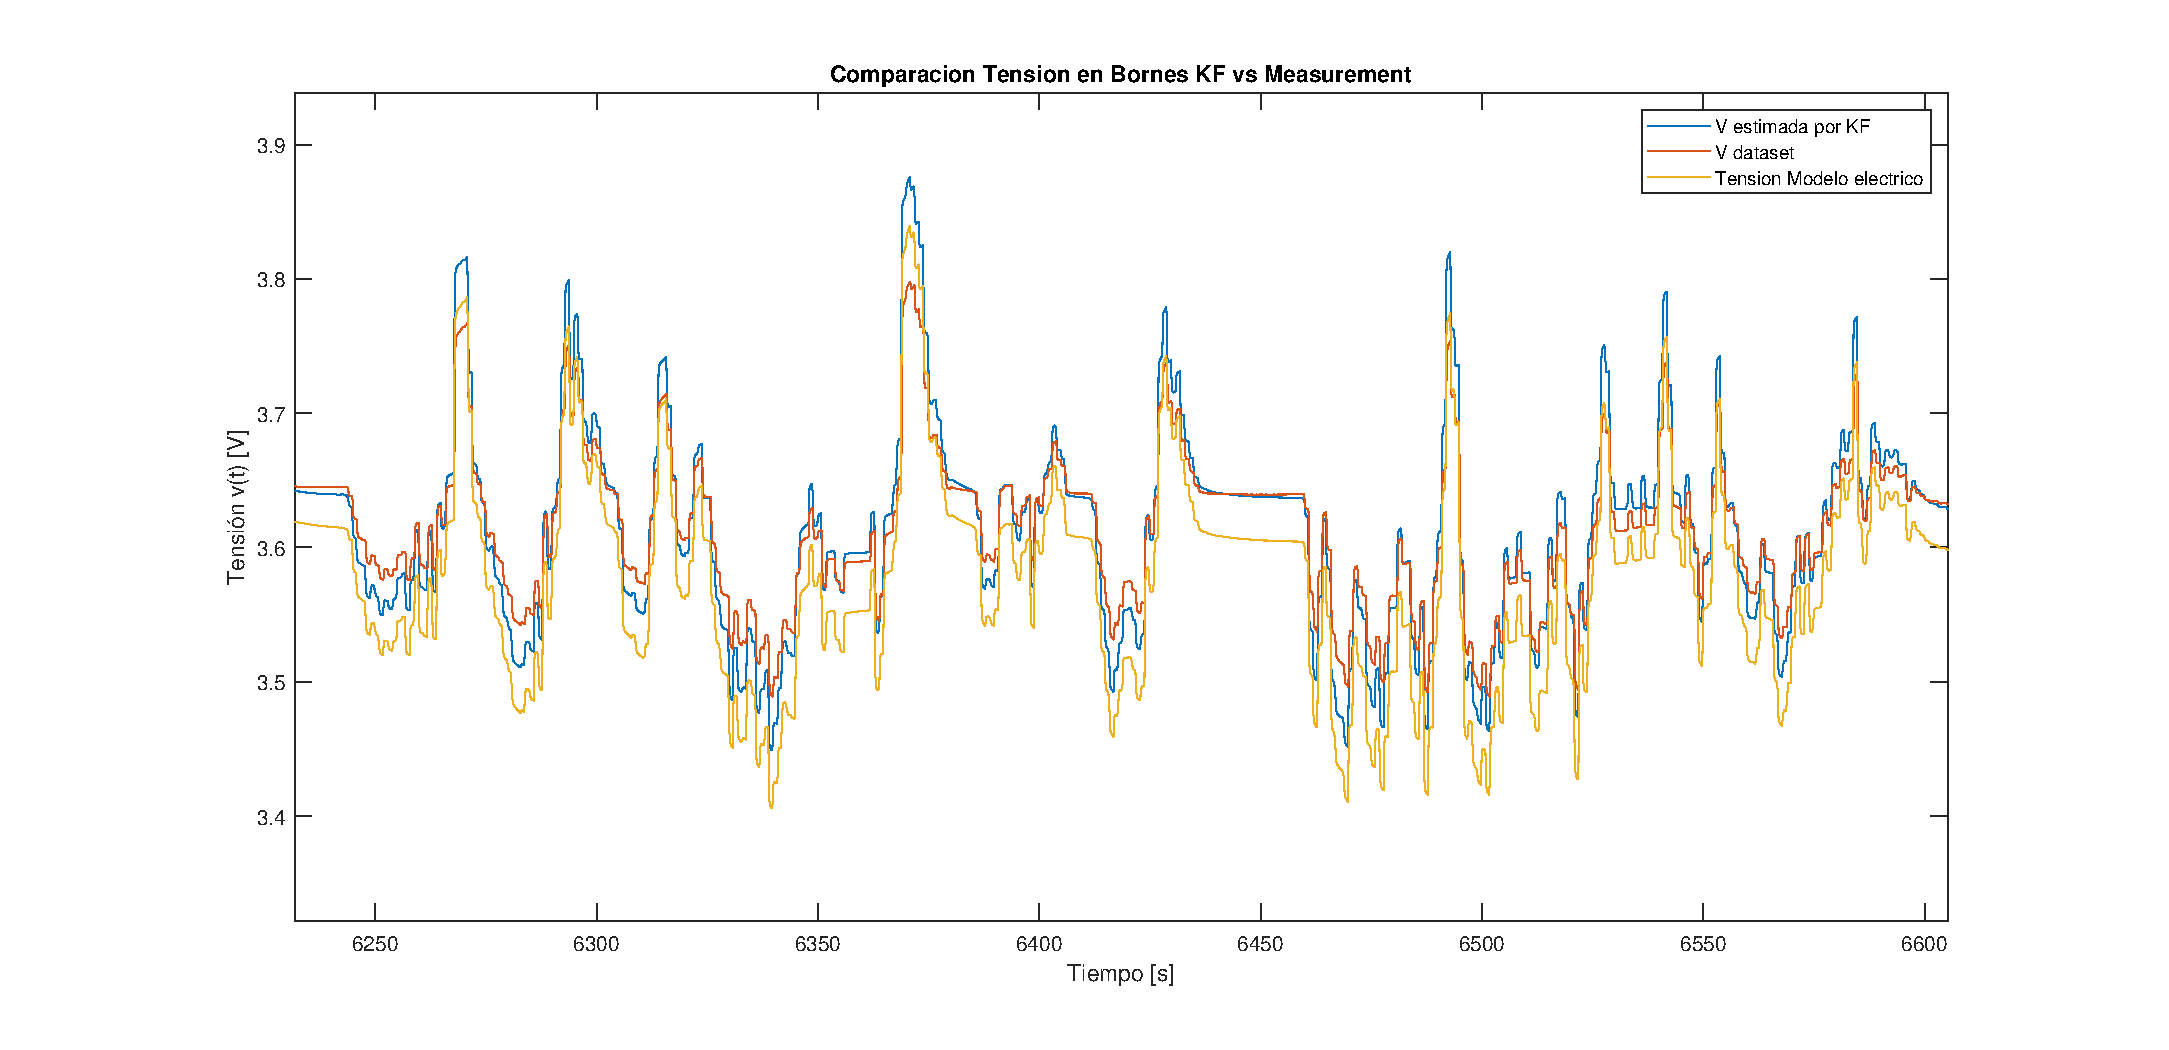
\includegraphics[width=1\textwidth]{Tension_Sim_zoom.eps}
			\caption{Detalle de la Simulación de la tensión en bornes de la 
                     batería sometida a condiciones de ciclo de manejo}
			\label{Tension_sim_zoom}
		\end{center}
	\end{figure}
	
	\clearpage 

	\noindent Si se presta especial atención el error se mantiene en una cota 
    del 6\% hasta que se dispara en la región de SoC menor al 15\% donde el 
    sistema se vuelve fuertemente alineal y nuestro modelo pierde validéz. 
    Por otro lado cumple satisfactoriamente con la corrección del SoC inicial 
    ya que estaba seteado en 20\% y el filtro corrige rapidamente a un valor 
    aproximado de 100\%. 
	
	\begin{figure}[h!]
		\begin{center}
			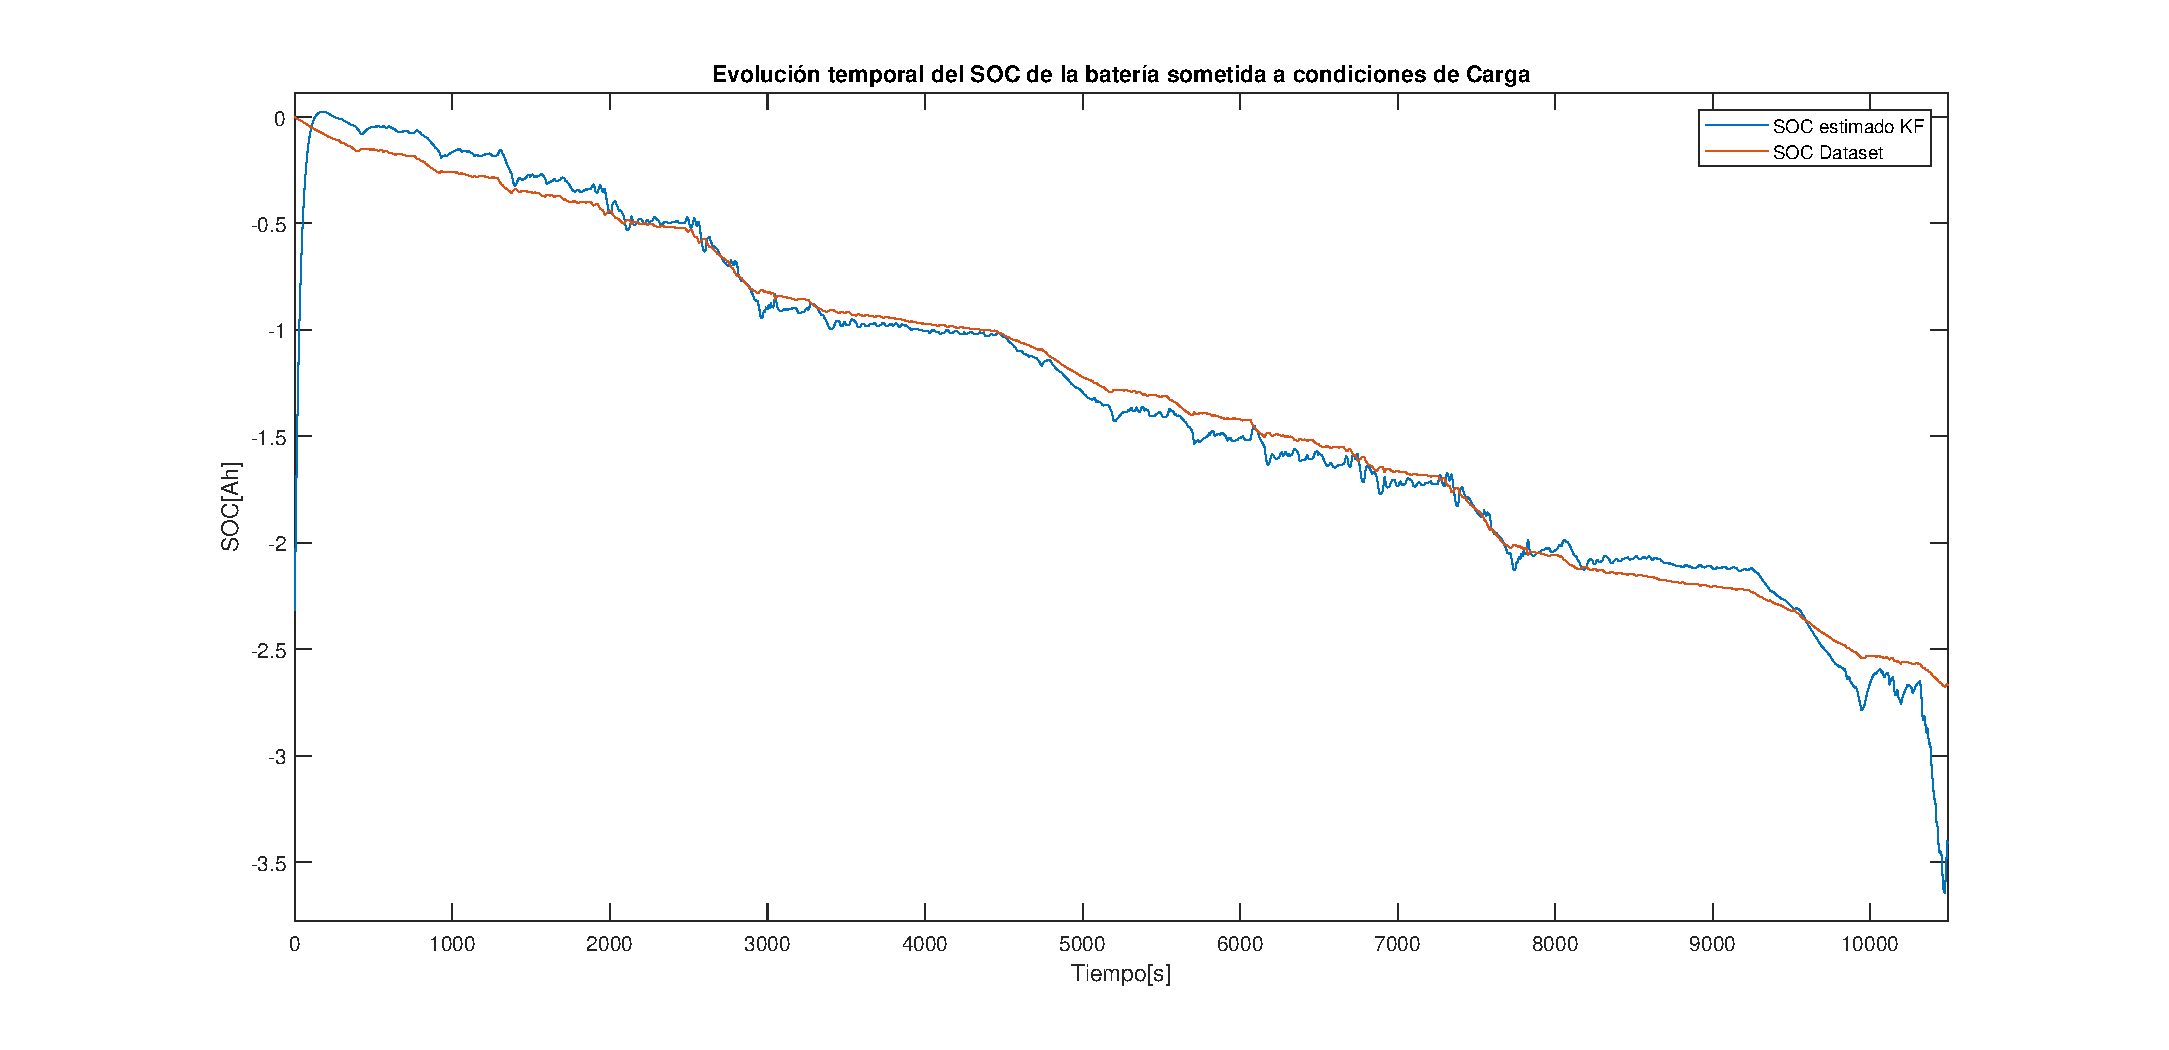
\includegraphics[width=1\textwidth]{Drive_Cycle_1_sim.eps}
			\caption{Resultados de la Simulación del sistema sometido a 
                     condiciones de ciclo de manejo}
			\label{Drive_Cycle_1_SoC_sim}
		\end{center}
	\end{figure}
	
	\begin{figure}[h!]
		\begin{center}
			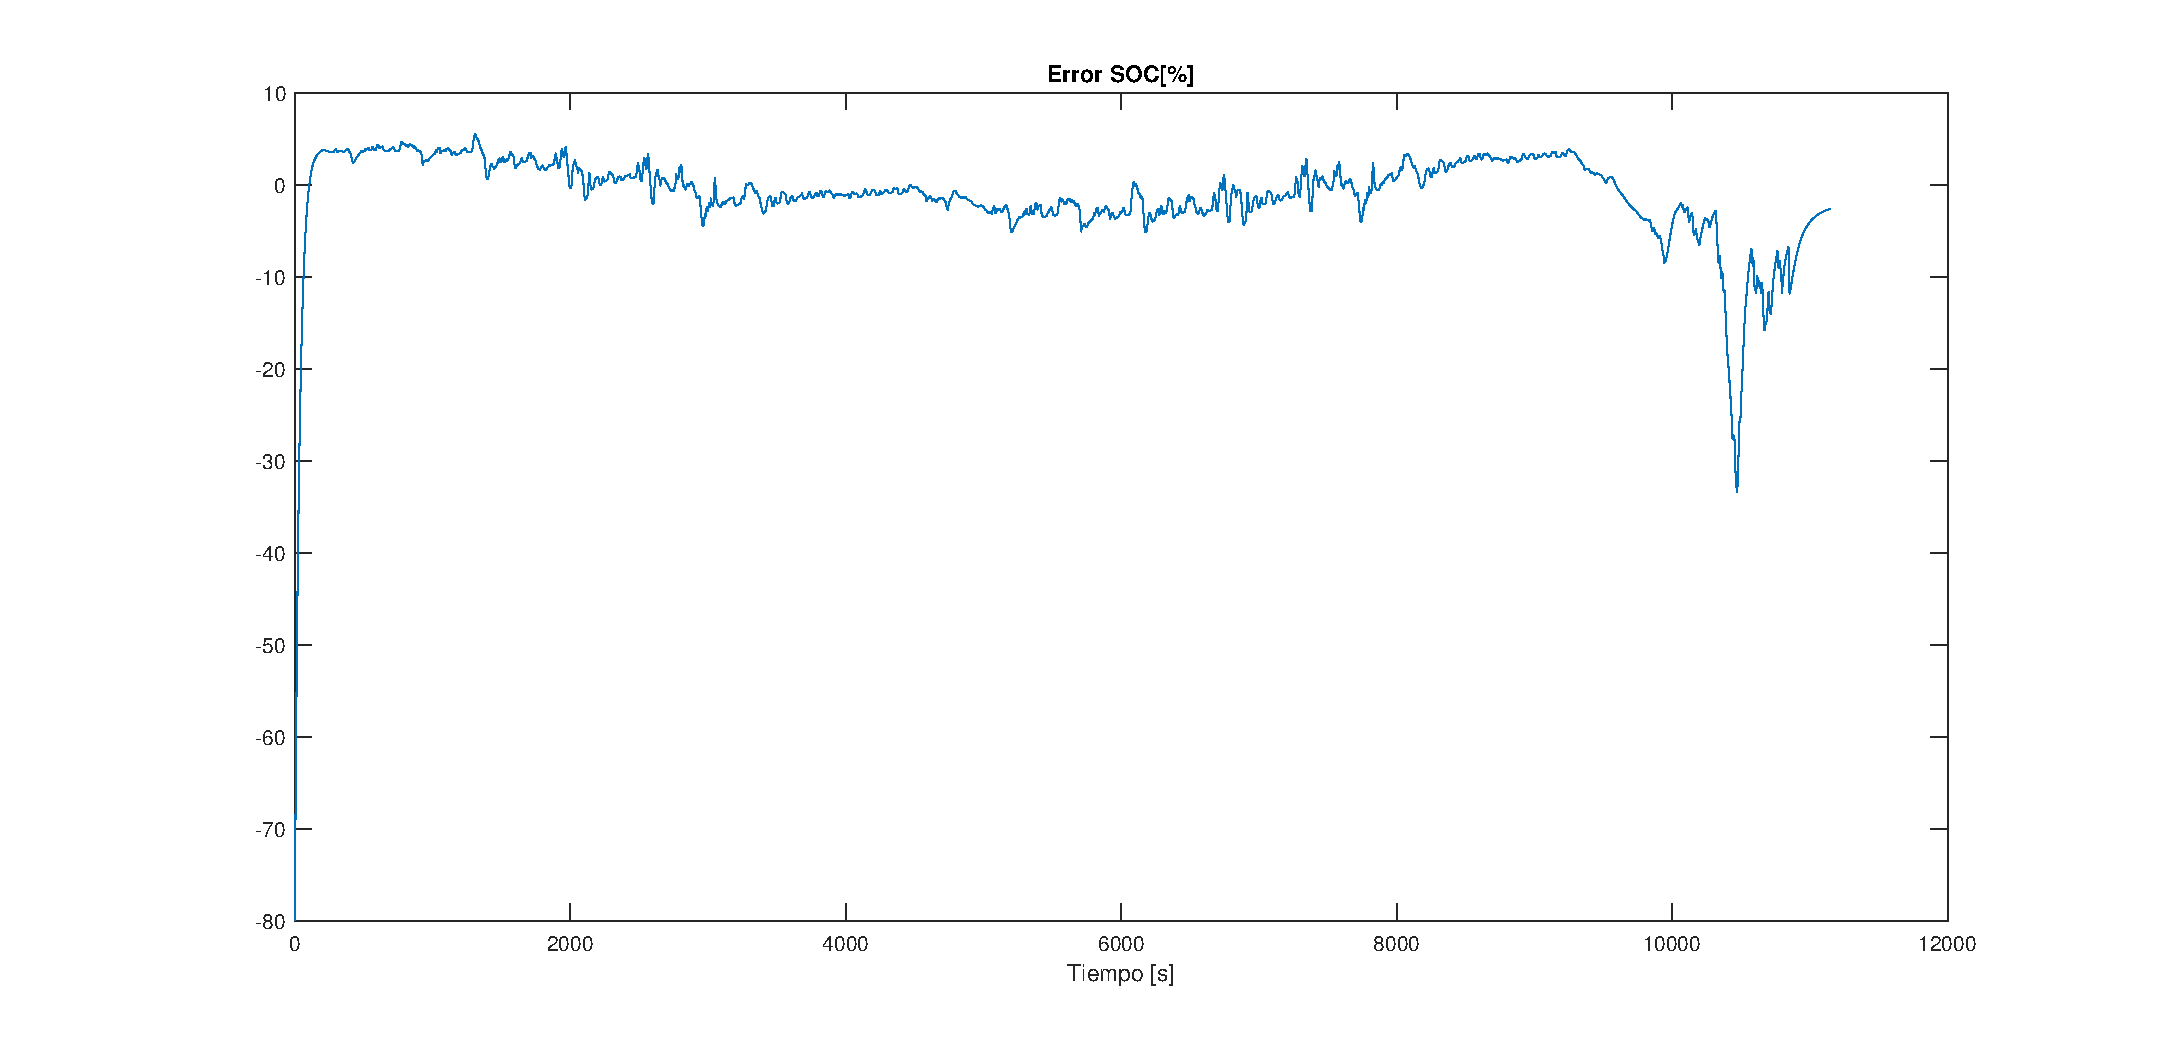
\includegraphics[width=1\textwidth]{soc_error_porc.eps}
			\caption{Resultados de Simulación del SoC de una batería sometida a 
                     condiciones de ciclo de manejo}
			\label{error_SoC_Sim}
		\end{center}
	\end{figure}
	
	\clearpage
	
	\subsection{Ecualización de celdas}
	
	Como se comentó en secciones anteriores, cuando múltiples celdas 
    se encuentran conectadas en serie, el voltaje de una celda no siempre 
    coincide con la tensión equivalente del pack de baterías dividido por el 
    número de celdas. 
	
	\noindent La ecualización de celdas es una técnica en la cual se trata de 
    mantener los niveles de voltaje entre las celdas que conforman la cadena 
    conectada en serie de un pack de baterías de forma homogénea, es decir, que 
    los niveles de tensión entre celdas sea lo más uniforme posible, con el 
    objetivo de maximizar la eficiencia del pack de baterías.
	
	\noindent El desbalance más típico generalmente se manifiesta en una 
    variación en el voltaje entre éstas, que puede ser corregido 
    instantáneamente o gradualmente conectando cargas externas en paralelo, a 
    través de sus correspondientes transistores, provocando una corriente de 
    descarga adicional que pueden ir desde miliamperes hasta varios Amperes, 
    dependiendo del dimensionamiento energético del pack de baterías. 
    Sin embargo, este desbalance en tensión es, por lo general, dado por 
    desbalances químicos o distintas dinámicas de descarga entre celdas, 
    provocando que el objetivo del balanceo no esté claramente definido 
    resultadno en más perjuicios que beneficios al sistema completo. 
    De hecho, la mayoría de las metodologías basadas en el desbalance de 
    voltaje, llevan a un pack de baterías más desbalanceado que sin ellos.

	\noindent Por lo tanto es necesario conocer la naturaleza de los distintos 
    tipos de desbalances, los cuales son descriptos a continuación:
	%\noindent Por lo tanto, existen varios tipos de desbalances que se describen a continuación.
	
	\subsubsection{Desbalance del estado de carga (SoC)}
	
	\noindent El desbalanceo por estado de carga es causado por celdas que son 
    cargadas a distintos nivels de SoC. Por ejemplo, si tenemos 3 celdas cuya 
    carga máxima es de 2200mAh ($\mathrm{Q_{max}}$), y descargar 100mAh una de 
    las celdas ($\mathrm{Q_1}$), la segunda por 100mAh y la tercera por 200mAh, 
    la primer y segunda celda van a estar a un SoC de 
    $\mathrm{\frac{(Q_{max} - Q_1)}{Q_{max}} = 95.4\%}$. pero la tercer celda 
    estará, a cálculo hecho, en un 91\%. Por lo que podemos decir que la tercer 
    celda presenta un desbalance de un 4.4\%. Esto se traduce en distintos 
    voltajes de circuito abierto, ya que se encuentran directamente 
    correlacionadas con el estado de carga de las mismas, sin embargo, a pesar 
    de esta diferencia constante de SoC, la tensión entre celdas varía con el 
    SoC debido a su variación con respecto a los distintos niveles de estado de 
    carga. En la Figura \ref{diff_imbalance} se muestra como varía la diferencia 
    de voltaje entre las celdas ante distintos niveles de SoC con un desbalance 
    constante teniendo en cuenta la curva de la figura 
    \ref{OCV_SoC_equalization_figure}.
	
	\begin{figure}[h!]
		\begin{center}
			\includegraphics[width=0.7\textwidth]{SoC_vs_OCV_equalization.png}
			\caption{(Gráfica superior): OCV vs SoC}
			\label{OCV_SoC_equalization_figure}
		\end{center}
	\end{figure}
	
	\clearpage 
	
	\begin{figure}[h!]
		\begin{center}
			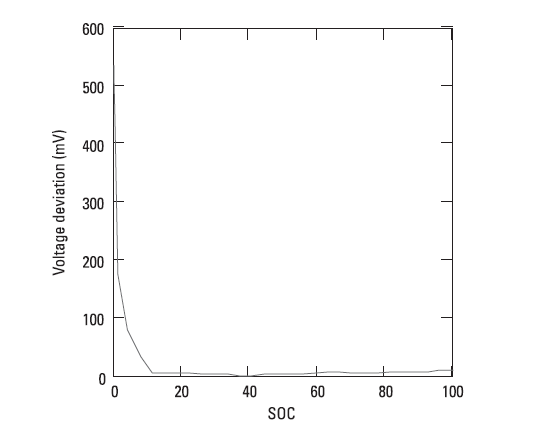
\includegraphics[width=0.7\textwidth]{diff_imbalance.png}
			\caption{Diferencia de OCV a distintos estados de carga para un desbalance de 1\% de SoC}
			\label{diff_imbalance}
		\end{center}
	\end{figure}
	
	\noindent El voltaje sobre una carga puede ser aproximadamente, 
    y rápidamente, modelada por la siguiente ecuación:
	
	\begin{equation}
		V = OCV(SoC) + I \times R(SoC)
		\label{v_load_bat}
	\end{equation}
	
	\noindent Debido a que la función $R(SoC)$ incrementa rápidamente a bajos 
    valores de SoC, la diferencia de voltajes entre celdas, con un desbalance 
    de SoC determinado, incrementa en un estado de carga muy bajo sugeriendo 
    que existe un incremento en la necesidad de realizar el proceso de balanceo 
    cuando el pack de baterías alcanza su descarga completa, sin embargo, 
    si esta diferencia de SoC es eliminada en etapas anteriores, las diferencias 
    de tensión que ocurren cerca del fin de descarga son eliminadas sin 
    necesidad de altas corrientes de drenaje para cada celda.
	
	\clearpage

	\subsubsection{Diferencias entre impedancias internas}
	
	La diferencia entre impedancias internas en un bache de producción es de 
    aproximadamente un 15\% como se puede observar en la Figura \ref{zin_diff}.
	
	\begin{figure}[h!]
		\begin{center}
			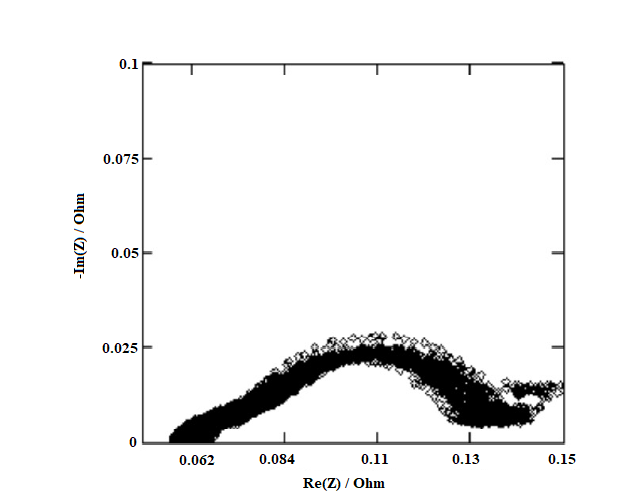
\includegraphics[width=0.7\textwidth]{zin_diff.png}
			\caption{Diferencias de espectrometrías entre 50 celdas. 
                     El ensayo es realizado entre 1kHz a 10mHz}
			\label{zin_diff}
		\end{center}
	\end{figure}
	
	\noindent Desbalances en la impedancia interna de la celda no causan 
    diferencias en el OCV, sin embargo, causará diferencias en el voltaje de la 
    celda durante la descarga, ya que la misma viene dada por la Ecuación 
    \ref{v_load_bat}. Si la batería se encuentra descargando, es decir, si 
    la corriente es negativa el voltaje que entrega a la carga será menor para 
    una celda con mayor impedancia interna. Por el otro lado, si la celda se 
    encuentra cargando, el voltaje será mayor para aquellas celdas con mayor 
    resistencia interna.
	
    \noindent A pesar de estas diferencias, no hay mecanismo de balanceo que 
    permita solventar el problema del desbalanceo de impedancia interna, ya que 
    no es manifiesto de un desbalanceo de carga, si no, mas intrinseco al 
    apareamiento entre las mismas.
	
	\subsubsection{Diferencias en la Capacidad de las celdas}
	
	Por el otro lado, puede suceder que la capacidad química de las celdas 
    ($\mathrm{Q_{MAX}}$) pueden ser diferentes en un principio, esto provoca 
    que, a pesar de que cada celda sea descargada por la misma cantidad de 
    corriente, el estado de carga será diferente. Por ejemplo, si las 3 celdas 
    que nombramos anteriores son descargadas por 100mAh, pero la 3er celda 
    tiene una capacidad distinta al resto (por ejemplo, 2000mAh en vez de 
    2200mAh), los estados de carga resultantes serán de 95.4\% y 95\%.
	
	Nuevamente esto provocará una diferencia en los OCVs de las celdas. 
    Como puede observarse, 200mAh de diferencia en $\mathrm{Q_{MAX}}$ causa 
    solamente una diferencia de un 0.4\% en el SoC, causando menor diferencia de 
    voltaje que un desbalance en el estado de carga.
	
	Teniendo esto en cuenta las baterías no podrán estar balanceadas durante 
    todo el ciclo de descarga o de carga ya que al quitar la misma cantidad de 
    carga el SoC de las mismas será distinto. Un ejemplo algo más gráfico de 
    esto es con 2 vasos de agua, uno con el doble de capacidad del otro pero 
    llenos hasta la misma altura. Si se remueve la misma cantidad de agua de 
    ambos el de mayor capacidad se habrá descargado la mitad que el de menor 
    capacidad.
	
	En la práctica lo más común es lo que se llama \emph{top balancing}, que 
    implica balancear en el período de carga en la que el pack se considera
    cargado a un 100\% o durante el periodo de Tension constante o CV (del
    ingles \emph{Constant Voltage}). El mismo consiste descargar las celdas de 
    menor capacidad permitiendo a las celdas de mayor capacidad un margen para 
    seguir cargando sin sobrecargar las primeras, evitando lo que generaría una 
    drástica disminución de la vida útil del pack. Esta opción es mucho más 
    atractiva que su contra parte denominada \emph{bottom balancing} ya que 
    esta balancea todas las baterías a su estado de carga cercano al 0\%, lo 
    cual no acarrea ninguna ventaja ya que el pack de baterías va a seguir 
    entregando a la carga la misma cantidad de energía, esto es, cuando la 
    batería de menor capacidad se descargue como pasaría si no se realizara el 
    balanceo inferior.
	
	
	La descarga de las celdas se puede llevar a cabo disipando su energía en 
    resistores o transfiriendo la carga a las celdas más descargadas, 
    siendo estos métodos clasificados como balanceo pasivo o balanceo activo 
    respectivamente. Los métodos pasivos son mucho más sencillos y económicos y 
    en la mayoría de los casos no es justificado el uso del método activo ya que 
    los circuitos que llevan a cabo la transferencia de energía poseen perdidas 
    por lo que no ofrecen ventajas reales en aplicaciones de baja potencia.
	
	Por último hay que considerar que corriente es necesaria para balancear el 
    pack, a mayor capacidad de corriente las corrientes de auto descarga y 
    cambios en la capacidad por envejecimiento van generando pequeños desbalances, 
    pero los mismos son acotados, las corrientes de auto descarga generan 
    desbalances menores al 0.1\% por ciclo. 
	
	\begin{figure}[h!]
		\begin{center}
			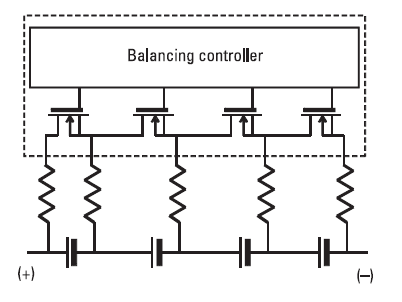
\includegraphics[width=0.7\textwidth]{passive_equalizator.png}
			\caption{Esquemático de conexión de un balanceador pasivo.}
			\label{passive_equalizator}
		\end{center}
	\end{figure}
	
	%Para la implementación del balanceador analizó LTC6803-2.\\

	El integrado BQ76PL536 de texas instrument es un Monitor de batería con 
    protecciones para sobre y baja tensión y sobrecalentamiento asi como también 
    posee varias funcionalidades entre las cuales se destacan la posibilidad de 
    escalar el número de celdas en serie gracias a su interfaz D2D VBUS 
    (\emph{device to device vertical BUS}) permitiendo la conexión en serie de 
    varios BQ76PL536 permitiendo controlar hasta un total de 192 celdas
    conectadas en serie.

	
	\clearpage
	\subsection{Plan de Trabajo}
	
	Se plantea el siguiente plan de trabajo con el tiempo estimado para la 
    finalización del proyecto:
	
	\begin{table}[h!]
		\begin{tabular}{|l|c|}
			\hline
			\multicolumn{1}{|c|}{Tarea}                                                                                                                                                                              & Duración                           \\ \hline
			\begin{tabular}[c]{@{}l@{}}Estudio, análisis y comparación del estado del arte de la tecnología. \\Estudio de los requerimientos de hardware.\end{tabular}                         & 2 Semanas                          \\ \hline
			\begin{tabular}[c]{@{}l@{}}Modelado de baterías de Li-Ion en MatLab. \\Simulación de los distintos algoritmos y los circuitos de protección. \\ Estudio y comparación. Validación y elección de los más adecuados.\end{tabular} & 4 Semanas                          \\ \hline
			\begin{tabular}[c]{@{}l@{}}Desarrollo e implementación del hardware del BMS. *\end{tabular}                                                      & 6 Semanas                          \\ \hline
			\begin{tabular}[c]{@{}l@{}}Desarrollo del Firmware del BMS con los algoritmos seleccionados.\\  Implementación y depuración sobre el hardware.\end{tabular}                                                    & 4 semanas                          \\ \hline
			Montaje del banco de pruebas para ensayar las protecciones y los algoritmos correspondientes. *                                                                                                                       & 3 Semanas                          \\ \hline
			Análisis de resultados, obtención de conclusiones y desarrollo del informe final.                                                                                                                                                       & 3 Semanas                          \\ \hline
			\textbf{Total}                                                                                                                                                                                                  &\textbf{24 Semanas} \\ \hline
		\end{tabular}
	\end{table}
	
	\subsection{Extensión a futuros proyectos}
	
	El desarrollo del hardware y los algoritmos, tanto de ecualización como de 
    estado de carga sirven como una buena base para futuros proyectos vinculados 
    a la temática de energías renovables y VEs.

	Como posible extensión se plantea el desarrollo de algoritmos novedosos para 
    la estimación del Estado de Salud o SoH (del ingles \emph{State of Health}), 
    su posible aplicación a sistemas de alta potencia e inclusive realizar 
    estudios sobre nuevas tecnologías relacionadas a la composición química de 
    las celdas.
	
	\clearpage
	
	\section{Bibliografía}
	
	\bibliography{Bms_Documentation} 
	\bibliographystyle{ieeetr}
	
\end{document}
